\documentclass[format=acmsmall, review=false]{acmart}
\makeatletter
\def\@ACM@checkaffil{% Only warnings
    \if@ACM@instpresent\else
    \ClassWarningNoLine{\@classname}{No institution present for an affiliation}%
    \fi
    \if@ACM@citypresent\else
    \ClassWarningNoLine{\@classname}{No city present for an affiliation}%
    \fi
    \if@ACM@countrypresent\else
        \ClassWarningNoLine{\@classname}{No country present for an affiliation}%
    \fi
}
\makeatother

\usepackage{acm-ec-23}
\usepackage{booktabs} % For formal tables
\usepackage[ruled]{algorithm2e} % For algorithms
\renewcommand{\algorithmcfname}{ALGORITHM}
\SetAlFnt{\small}
\SetAlCapFnt{\small}
\SetAlCapNameFnt{\small}
\SetAlCapHSkip{0pt}
\IncMargin{-\parindent}

% Choose a citation style by commenting/uncommenting the appropriate line:
\setcitestyle{acmnumeric}
% \setcitestyle{authoryear}

\usepackage{framed} 
\usepackage{amsthm}
\usepackage{tikz}
\usepackage{multirow}
\usepackage{pifont}
\usepackage{subfigure}
\usetikzlibrary{patterns,patterns.meta}
\usetikzlibrary {arrows.meta}
% Title. Note the optional short title for running heads. In the interest of anonymization, please do not include any acknowledgements.
\title[]{Connected Trading Cycles}

\author{Xinwei Song}
\author{Tianyi Yang}
\author{Dengji Zhao}
\affiliation{
\institution{Shanghaitech University}
\country {China} % adding country macro
}


% Abstract. Note that this must come before \maketitle.
\begin{abstract}
This paper studies one-sided matching with initial endowments and the social connections between participants are specifically considered (their social network). Different from the traditional setting, the matching starts with a group of initial participants, and the others need their invitation to join the matching game. Thus, the incentive compatibility (IC) notion here considers both reporting preferences and inviting others via their social connections. This is challenging because inviters and invitees might compete in the game. Besides IC, stability and optimality are two properties extensively studied in matching, but they both are incompatible with the new IC. In the new setting, compatible stability has been discussed, but no discussion about compatible optimality yet. We complete this and prove the theoretical boundaries regarding both stability and optimality in the new setting. We then propose a mechanism called Connected Trading Cycles to satisfy all the desirable properties for the first time. Unlike the previous solutions that add restrictions on participants' matching choices to achieve IC, we allow participants to choose anyone in the game, which in principle improves everyone's satisfiability in the matching. Finally, we give the first characterization of IC in the network setting to facilitate IC mechanism design. 

%Furthermore, we give a a family of social networks which guarantees the tightness of the theoretical boundaries. For completeness, we provide a graph transformation procedure which can transform any social network to the family which guarantees the tightness of properties. 
%In this way, all the players benefit from the invitation. 
 %which is based on participants' connections and trading cycles
%Finally, we conduct simulations to compare currently existing IC one-sided matching mechanisms and analyze their cardinal performance. We adopt three criteria to distinguish our solution from the others and discuss the value of achieving optimality.
%We also find that the monotonicity in each dimension is the sufficient and necessary condition for an IC mechanism.
\end{abstract}
\begin{document}

% Title page for title and abstract only.
\begin{titlepage}

\maketitle

\end{titlepage}

\section{Introduction}
Mechanism design on social networks is a new trend~\cite{DBLP:conf/atal/Zhao21}. It specifically models the participants' social connections in various games including matching, auctions and cooperative games. The social connections are private information for each participant, and those who are already in the game can decide whether or not to invite their direct neighbors. The primary purpose of this new study is to utilize participants' social connections to expand the markets for better outcomes. In matching, more participants will give more matching choices and lead to a more satisfying matching outcome. 
%Several real-world applications like online housing market\footnote{https://www.homeexchange.com, https://www.lovehomeswap.com} and second-hand goods exchange platforms\footnote{https://www.freecycle.org} have applied this idea and become successful business models. In these platforms, former participants propagate the information to their social networks to invite friends and form a credible market. 
This is essentially very useful to promote a game on a social network and to inspire new applications utilizing social platforms (such as online housing market\footnote{https://www.homeexchange.com, https://www.lovehomeswap.com} and second-hand goods exchange markets\footnote{https://www.freecycle.org}).
%(such as a second hand goods exchange market) 
However, inviting others is not always beneficial. %invitation incentives do not come easily because the invitees may be a threat to their inviters. 
Let's consider a simple example that might happen in a house exchange game. Suppose there are two initial users, Alice and Bob. As shown in Figure~\ref{fig:Driving}(a), Alice and Bob prefer each other's house and they will exchange if there is no other choice. Assuming Alice has a friend Charlie, Bob and Charlie will prefer to exchange with each other if three of them are in the game (Figure~\ref{fig:Driving}(b)). As a result, Alice will not invite Charlie if Charlie is not in the game yet.
 %who likes Bob's house and owns a house that Bob prefers over Alices's, her dominant strategy is to maintain the Alice-and-Bob market instead of inviting Charlie. Otherwise, she may risk losing Bob's house as shown in Figure~\ref{fig:Driving} (b).
\begin{figure}[ht]
\centering
\subfigure[Initial Market]{
\centering
\begin{minipage}[ht]{0.3\linewidth}
\centering
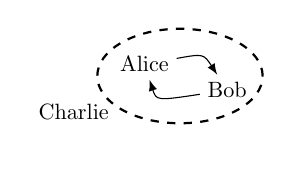
\begin{tikzpicture}[scale=0.3, sibling distance=5em,
  every node/.style = {scale=0.8, shape=rectangle, draw=none, align=center},
    outline/.style={draw=#1,thick,fill=#1!100}]
  every draw/.style = {scale=1}
  
  \draw[color=white,thick,dashed] (3.6,7.5) ellipse (5 and 2.5);
  \draw[color=black,thick,dashed] (5,8.5) ellipse (3.5 and 2);
  \node[color=black] (node1) at (3.5,9) {Alice};
  \node[color=black] (node2) at (7,7.9) {Bob};
  \node[color=black] (node3) at (0.5,7) {Charlie};
  % \draw[-] (node1)--(node3);
  \draw[-latex] (node1).. controls(6,9.45) ..(node2);
  \draw[-latex] (node2).. controls(4,7.45) ..(node1);
\end{tikzpicture}
\end{minipage}
}
\subfigure[Inviting Charlie]{
\centering
\begin{minipage}[ht]{0.3\linewidth}
\centering
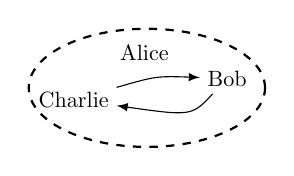
\begin{tikzpicture}[scale=0.3, sibling distance=5em,
  every node/.style = {scale=0.8, shape=rectangle, draw=none, align=center},
    outline/.style={draw=#1,thick,fill=#1!100}]
  every draw/.style = {scale=1}
  \draw[color=black,thick,dashed] (3.6,7.5) ellipse (5 and 2.5);
  \node[color=black] (node1) at (3.5,9) {Alice};
  \node[color=black] (node2) at (7,7.9) {Bob};
  \node[color=black] (node3) at (0.5,7) {Charlie};
  % \draw[-] (node1)--(node3);
  \draw[-latex] (node2).. controls(5.5,6.3) ..(node3);
  \draw[-latex] (node3).. controls(4,8) ..(node2);
\end{tikzpicture}
\end{minipage}
}
\caption{Driving Example }
\label{fig:Driving}
\end{figure}

According to the example, we can see that participants have the power to selectively invite others for their own interests. Thus, the main obstacle for mechanism design in the network setting is to provide incentives for participants to invite all their neighbors to join the game. In auctions, we can pay the harmed inviters some rewards~\cite{li2022diffusion}. In cooperative games, we can let the inviters share their invitees' contributions~\cite {zhang2022incentives}. Matching as a non-monetary game faces a greater challenge since the mechanism cannot compensate for the loss caused by invitation through payments. 
%There have been a few studies focusing on one-sided matching over social networks, especially the housing market and its variant~\cite{DBLP:conf/atal/KawasakiWTY21,tenants_social_network,Leave_and_Share}. 

To evaluate a matching mechanism, optimality and stability are two crucial properties. The former characterizes how good a matching is while the latter depicts the robustness of a matching, i.e., whether participants have incentives to deviate from the matching and exchange in a smaller group. The Top Trading Cycles (TTC) presented by~\citeauthor{shapley1974cores}~\cite{shapley1974cores} is proved to be the only Pareto optimal and stable mechanism for one-sided matching with endowments~\cite{ma1994strategy}. However, TTC cannot work in the social network setting due to the lack of invitation incentives. As shown by \citeauthor{kumar2022integration}~\cite{kumar2022integration}, more than half of the participants tend to form a smaller market under TTC. 
In the network setting, participants can decide the size of the market through strategic invitations, which causes the incompatibility between IC, stability, and optimality. 
Hence, it is valuable to understand what else we can achieve with IC near stability or optimality~\cite{DBLP:conf/atal/KawasakiWTY21,Leave_and_Share}.

%In the traditional setting, mechanism designers do not need to take this into consideration, since the market size is irrelevant to participants' actions. 
%Hence, we should investigate new theoretical boundaries and design a mechanism to reach them.



Previous work has defined a new notion of stability under the network setting and has designed mechanisms to achieve it~\cite{Leave_and_Share}. As far as we are concerned, no previous work has investigated the new notion of optimality compatible with IC in the network setting. Therefore, we propose new notions of optimality and prove their compatibility with IC and stability (Section 4). 
%Inspired by the new optimality notion, we push the theoretical boundary regarding stability one step further. We prove that our redefined stability is the tightest stability that is compatible with IC under a special family of graphs. For other graphs, we propose a graph transformation procedure, that can be equipped on any mechanism that satisfy the redefined optimality and does no affect its property regarding optimal, stable or IR, IC.
%Since there exists an impossibility of the coexistence of IC and Pareto optimality in the new setting~\cite{DBLP:conf/atal/KawasakiWTY21,Leave_and_Share}, we define achievable optimality that can coexist with IC by enlarging the `optimal allocation' set. 

%To achieve the redefined stability and optimality, 
Given the achievable notions of stability and optimality, we design an IC mechanism called Connected Trading Cycles (CTC) to satisfy them (Section 5). We concentrate on two features, trading cycles and social connections, which are the principles of one-sided matching and social networks respectively. An allocation in one-sided matching consists of several trading cycles among agents. The key is to let everyone point to her favorite item, so the correlated trading cycles ensure optimality and stability. However, whether a trading cycle can get formed and traded is determined by its corresponding social connections in the network. Intrinsically, in the network setting, the trading cycles should build on a particular group of agents who know each other through their social connections within the group. In this way, no one outside the cycle has the power to break the trading cycle. Following this principle, we combine two features together to design Connected Trading Cycles. Different from the previous solutions, we do not restrict agents' choice scope, and they can choose anyone in the game. 
%Combining the graph transformation procedure and CTC, we can have a mechanism which reaches the theoretical boundary of diffusion one-sided matching.

Finally, we give the first characterization of IC in the network setting (Section 7). We propose two monotonicity conditions that depict IC one-sided matching on networks to help mechanism designers construct and identify new IC solutions. 

%all desirable mechanisms with invitation incentives to refine/complete the theoretical framework. 

%In theory, only our solution can achieve both redefined stability and optimality, it is very interesting to see how it differs from the other solutions in terms of efficiency and participants' satisfaction. Therefore, we conduct experiments to analyze the differences.


\noindent\textbf{Our Contributions}
\begin{itemize}
    \item We prove the achievable notions/boundaries of stability and optimality with incentive compatibility for one-sided matching in the network setting. %We prove the theoretical boundaries and fill the gap regarding optimality in one-sided matching over social networks.
    \item We propose a new mechanism called Connected Trading Cycles that reaches the theoretical boundaries and dominates the existing mechanisms.
    \item We give the first characterization of incentive-compatible one-sided matching mechanisms in the network setting.
    %\item We conduct simulations to compare our mechanism with the previous mechanisms and analyze the differences from three perspectives.

\end{itemize}

%%%%%%%%%%%%%%%%%%%%%%%%%%%%%%%%%%%%%%%%%%%%%%%%%%%%%%%%%%%%%%%%%%%%%%%%

\section{Literature Review}

\citeauthor{li2017mechanism}~\cite{li2017mechanism} initiate the line of research on mechanism design over social networks. This new setting models the market in a dynamic way and makes use of the power of social networks to offer both the participants and the market owner a better outcome~\cite{DBLP:conf/atal/Zhao21}. In the social network setting, the classic solutions cannot work anymore because they fail to provide invitation incentives. For games with monetary transfers, like auctions and cooperative games, we can 
incentivize invitations to form a larger game by giving them rewards~\cite{li2022diffusion,zhang2022incentives}. However, when it comes to non-transferable utility games like matching, incentives for invitation are harder to design. 

In the network setting, the incentive compatibility notion for one-sided matching is defined in two dimensions. Due to the expansion of IC, the appropriate solution space for mechanism designers also changes. Thus, how to characterize the IC one-sided matching mechanisms in the network setting is an important problem. In literature, finding the characterization for desired properties has always been a rich research topic. \citeauthor{TAKAMIYA2001201}~\cite{TAKAMIYA2001201} characterizes the IC as well as the core solution for the housing market. Later on, \citeauthor{sonmez2010house}~\cite{sonmez2010house} study the characterization of a variant of the housing market. Seeking alternative depictions for TTC is also an active research field~\cite{sethuraman2016alternative,chen2021alternative,anno2015short}. These works provide insights for the mechanism designers and help them come up with better algorithms. In this paper, we present an IC characterization of the new setting.

For matching over social networks, designing invitation incentives can help enlarge the selection space and improve matching results for the participants. \citeauthor{DBLP:conf/atal/KawasakiWTY21}~\cite{DBLP:conf/atal/KawasakiWTY21} and \citeauthor{tenants_social_network}~\cite{tenants_social_network} degenerate social networks to trees and modify the classic mechanisms to incentivize invitations for housing market as well as its variant~\cite{abdulkadirouglu1999house}. Specifically, they add limits on the selection space of the participants in a tree to incentivize invitations. \citeauthor{Leave_and_Share}~\cite{Leave_and_Share} take a step forward and propose a mechanism that works for all networks. In their mechanism, participants can only choose from their current neighbor set, and their neighbor set is dynamically shared when participants leave the market. Due to the sharing process, their mechanism gives a more efficient outcome. For two-sided matching, \citeauthor{ijcai2022-27}~\cite{ijcai2022-27} model the school choice problem into the network setting and design invitation incentives for the student side only. Another thread of work also takes the social network and its influence into consideration, but they differ from our setting~\cite{DBLP:conf/ijcai/GourvesLW17,HOEFER201320}. In their setting, the social network is priorly known and acts as a constraint for possible allocations.


Besides incentive compatibility, optimality is another concerned property for one-sided matching mechanisms~\cite{abdulkadiroglu2013matching}. The celebrated TTC is the only Pareto optimal and stable solution in the traditional setting~\cite{ma1994strategy}. When it comes to the house allocation problem, optimal solutions are multiple. \citeauthor{abraham2004pareto}~\cite{abraham2004pareto} study various ways to evaluate the optimality of a house allocation mechanism and illustrate why TTC gives the Pareto optimal allocation. \citeauthor{fleischer2008dynamic}~\cite{fleischer2008dynamic} point out the transitions between different optimal allocations in the house allocation problem. \citeauthor{brandt2019convergence}~\cite{brandt2019convergence} analyze whether different types of dynamic pairwise swaps converge to Pareto optimal allocations for matching markets. However, no previous work has investigated achievable optimality in the network setting. To evaluate the efficiency of a mechanism, we need to redefine an optimality notion in the new setting. Hence, we construct a tight optimality notion and design a mechanism to reach it.

%Apart from Pareto optimality, there are other criteria to evaluate the optimality of a matching. Rank maximality is considered a more practical measurement for matching~\cite{irving2006rank}. It requires matching more agents with their top choice as possible, and it is widely used in applications like assigning papers to referees~\cite{Garg2009AssigningPT}. Moreover, we can also compare two matching mechanisms by their popularity, which is determined by the votes of the participants~\cite{abraham2007popular}.

%In matching, cardinal methods are widely used to evaluate the performance of a mechanism~\cite{anshelevich2010matching,bhalgat2011social,echenique2017ordinal}. There are also some studies investigating the trade-offs between achieving the desired properties and achieving a better cardinal result~\cite{boudreau2013preferences}. In Section 8, we will adopt a cardinal method to evaluate our solution, to see whether reaching the theoretical optimality comes at a cost.



%%%%%%%%%%%%%%%%%%%%%%%%%%%%%%%%%%%%%%%%%%%%%%%%%%%%%%%%%%%%%%%%%%%%%%%%

\section{The Model}
In this section, we model one-sided matching over social networks with formal definitions. A one-sided matching market consists of a set of agents $N=\{1,\dots, n\}$, each with an indivisible initial endowment, usually referred to as a house. We denote the set of endowments as $H=\{h_1,\dots, h_n\}$. Every agent $i$ has a strict preference $\succ_i$ over the endowment set $H$. Specifically, $h_j\succ_i h_k$ indicates agent $i$ prefers $h_j$ over $h_k$. We use $\succeq_i$ to represent a weak preference where $h_j\succeq_i h_k$ implies that agent $i$ strictly prefers $h_j$ over $h_k$, or $i$ is indifferent with $h_j$ and $h_k$. 
%For simplicity, the $a^{th}$ ranked item in agent $i$'s preference ($a\in Z \cap [1,n]$) is denoted by $\succ_i(a)$ . To present agent $i$'s preference over a subset of endowments $H'\subset H$, we use $\succ_i^{H'}$ to notate $i$'s truncated preference. 
To characterize the social network, we use an undirected graph $G=(N, E)$ to depict the social connections among agents in $N$. We say agents $i$ and $j$ are neighbors to each other if there exists an edge $(i,j)\in E$. Let $r_i$ represent the neighbor set of agent $i$, then $(i,j)\in E$ indicates $i\in r_j$ and $j\in r_i$. 

In our setting, the social network $G$ is not priorly known to anyone. Both the preference and the neighbor set are private information to each agent. We define a type profile $\theta_i=(\succ_i, r_i)$ for agent $i$, which consists of her preference $\succ_i$ and her neighbor set $r_i$. We denote the type profile for all agents as $\theta = (\theta_1,\dots,\theta_n)$ and $\Theta$ as the type profile space. Let $\theta_{-i}$ be the type profile without agent $i$, then we have $\theta = (\theta_{i},\theta_{-i})$. Analogously, $\Theta = (\Theta_{i},\Theta_{-i})$. We denote agent $i$'s reported type profile as $\theta'_i=(\succ'_i, r'_i), \theta'_i\in\Theta_i$. In practice, reporting one's neighbor set equals inviting one's neighbors to join the game. One cannot report a non-neighbor as her neighbor, because she does not know the others. Thus, we have $r'_i\subseteq r_i$ for each agent $i$. 

\begin{definition}
A one-sided matching mechanism is defined by an allocation policy $\pi = (\pi_i)_{i\in N}$, where $\pi_i:\Theta \to H$ satisfies for all $\theta \in \Theta$, for all $i$, $\pi_i(\theta) \in H$, and $\pi_i(\theta) \neq \pi_j(\theta)$ for all $i \neq j$.
\end{definition}

The above definition is the standard, and we need some constraints to cope with the two-dimensional type profile. Since the social connections are private information in our setting, a matching market over social networks usually starts with an initial set of agents $N_0\subset N$, who are the selected seed participants, or neighbors of the sponsor. The agents already in the market then report their type profile $\theta'$ to enlarge the market. With the reported profile $\theta'$, we construct the diffusion matching market as a directed graph $G(\theta')=(N(\theta'), E(\theta'))$, with $N(\theta')=\{1,\dots,n\}$ and $\langle i,j\rangle  \in E(\theta')$ indicates $j \in r'_i$. We define $Q(\theta')$ as the set of qualified agents who can participate in the matching and $N(\theta') \setminus Q(\theta')$ as the set of unqualified agents who stay outside of the diffusion market with their initial endowments. Note that agent $i\in Q(\theta')$ if and only if there exists a path from $N_0$ to $i$ in $G(\theta')$, which means $i$ is invited to the market by a series of invitations. Thus, all agents in $Q(\theta')$ forms a connected graph in $G(\theta')$.

\begin{definition}
A diffusion one-sided matching mechanism in social networks is a one-sided matching mechanism, $\pi = (\pi_i)_{i\in N}$, such that for all reported type profiles $\theta'\in\Theta$, it satisfies:
\begin{enumerate}
    \item for all unqualified agents $i\notin Q(\theta')$, $\pi_i(\theta') = h_i$.
    \item for all qualified agents $i\in Q(\theta')$, $\pi_i(\theta')$ is independent of the report of all unqualified agents.
\end{enumerate}
\end{definition}

We then define desirable properties for a diffusion one-sided matching mechanism. Firstly, to incentivize rational agents to join a game, a mechanism should at least guarantee joining in the game is not losing for each agent if she behaves truthfully. We call this property individual rationality.

\begin{definition}[Individual Rationality (IR)]
A diffusion one-sided matching mechanism $\pi$ is individually rational if for all $i\in N $, all $\theta_i \in \Theta_i$, and all $\theta'_{-i}\in \Theta_{-i}$, we have $\pi_i(\theta_i,\theta_{-i}')\succeq_i h_i$.
\end{definition}

Furthermore, incentivizing all agents to report their types truthfully is the key property of diffusion mechanisms. This requires that revealing true preference and inviting all neighbors to join in the game is a dominant strategy for all agents. We formulate this property as incentive compatibility.

\begin{definition}[Incentive Compatibility (IC)]
A diffusion one-sided matching mechanism $\pi$ is incentive compatible if for all $i\in N$, all $\theta'_{-i}\in \Theta_{-i}$ and all $\theta_i, \theta'_i\in \Theta_i$, we have $\pi_i(\theta_i,\theta'_{-i})\succeq_i \pi_i(\theta'_i,\theta'_{-i})$.
\end{definition}

For one-sided matching mechanisms, stability and Pareto optimality are used to measure the quality of the outcome. We formalize them for diffusion one-sided matching mechanisms as follows.

\begin{definition}[Stability]
A diffusion one-sided matching mechanism $\pi$ is stable if for all type profiles $\theta$ and the allocation $\pi(\theta)$, there is no agent set $S\subseteq N$ (with item set $H_S\subseteq H$) and another allocation $\pi'(\theta)$ with $\forall i \in S, \pi'_i(\theta)\in H_S$ such that $\forall i \in S, \pi'_i(\theta)\succeq_i\pi_i(\theta)$ and $\exists j \in S, \pi'_j(\theta)\succ_j\pi_j(\theta)$.
\end{definition}

Namely, a matching is stable if no coalition of agents wants to leave the matching to match alone.

% \begin{definition}[Pareto Optimality (PO)]
% A diffusion one-sided matching mechanism $\pi$ is Pareto optimal if for all type profiles $\theta$ and the correlated allocation $\pi(\theta)$, there is no other allocation $\pi'(\theta)$ such that $\exists T\subseteq N$, $\forall j \in T, \pi'_j(\theta) \succ_j \pi_j(\theta)$ and $\forall i\in N \setminus T$, $\pi'_i(\theta) = \pi_i(\theta)$.
% \end{definition}

\begin{definition}[Pareto Optimality (PO)]
A diffusion one-sided matching mechanism $\pi$ is Pareto optimal if for all type profiles $\theta$ and the allocation $\pi(\theta)$, there is no other diffusion one-sided matching mechanism $\pi'$ such that $\forall i \in N, \pi'_i(\theta) \succeq_i \pi_i(\theta)$ and $\exists T\subseteq N, T \neq \emptyset$, $\forall j \in T, \pi'_j(\theta) \succ_j \pi_j(\theta)$.
\end{definition}

The above definition of PO is an equivalent form of that in the traditional model. The reason why we define PO this way is for the simplicity of its extensions in the network setting. 

\citeauthor{Leave_and_Share}\cite{Leave_and_Share} prove that these two properties are not compatible with IC and IR in the social network setting. For stability, they propose that the group who deviate and swap among themselves be a connected component or a complete component to define weaker notions. They show that stable under complete components is compatible with IC. We apply the same notions here.

%in social network setting and even a slight ease of the limit fails to be compatible with IC.

%in the social network and define stable under connected components, stable under complete components respectively. 
\begin{definition}[Stability under Connected Components (Stable-c)]
A diffusion one-sided matching mechanism $\pi$ is stable under connected components if for all type profiles $\theta$ and the allocation $\pi(\theta)$, there is no agent set $S\subseteq N$ (with item set $H_S\subseteq H$), that forms a \textbf{connected component} in $G(\theta)$, and another allocation $\pi'(\theta)$ with $\forall i \in S, \pi'_i(\theta) \in H_S$ such that $\forall i \in S, \pi'_i(\theta)\succeq_i\pi_i(\theta)$ and $\exists j \in S, \pi'_j(\theta)\succ_j\pi_j(\theta)$.
\end{definition}


\begin{definition}[Stability under Complete Components (Stable-cc)]
A diffusion one-sided matching mechanism $\pi$ is stable under complete components if for all type profiles $\theta$ and the allocation $\pi(\theta)$, there is no agent set $S\subseteq N$ (with item set $H_S\subseteq H$), that forms a \textbf{complete component} in $G(\theta)$, and another allocation $\pi'(\theta)$ with $\forall i \in S, \pi'_i(\theta) \in H_S$ such that $\forall i \in S, \pi'_i(\theta)\succeq_i\pi_i(\theta)$ and $\exists j \in S, \pi'_j(\theta)\succ_j\pi_j(\theta)$.
\end{definition}


For optimality, we follow the new notions of stability and do a similar relaxation. By definition, Pareto optimality requires that the allocation cannot improve without making anyone worse off. Intuitively, we can regard the Pareto improvement as a reallocation process posterior to a certain allocation. In such way, we require those who can be reallocated should at least have a path to their reallocated items. Therefore, we further require the improved agents to be a connected component or a complete component to weaken optimality. 
%if we regard the blocking coalition as an allocation process prior to a certain allocation, 

%and define optimality under connected components, optimality under complete components respectively.
\begin{definition}[Optimality under Connected Components (Optimal-c)]
A diffusion one-sided matching mechanism $\pi$ is optimal under connected components if for all type profiles $\theta$ and the allocation $\pi(\theta)$, there is no other diffusion one-sided matching mechanism $\pi'$ such that $\forall i \in N, \pi'_i(\theta) \succeq_i \pi_i(\theta)$ and $\exists T \subseteq N, T \neq \emptyset $, $\forall j \in T, \pi'_j(\theta) \succ_j \pi_j(\theta)$ and $T$ forms a \textbf{connected component} in $G(\theta)$. 
\end{definition}


\begin{definition}[Optimality under Complete Components (Optimal-cc)]
A diffusion one-sided matching mechanism $\pi$ is optimal under complete components if for all type profiles $\theta$ and the allocation $\pi(\theta)$, there is no other diffusion one-sided matching mechanism $\pi'$ such that $\forall i \in N, \pi'_i(\theta) \succeq_i \pi_i(\theta)$ and $\exists T\subseteq N, T \neq \emptyset$, $\forall j \in T, \pi'_j(\theta) \succ_j \pi_j(\theta)$ and $T$ forms a \textbf{complete component} in $G(\theta)$. 
\end{definition}

% Inspired by our redefined optimality notion, we define a new stability notion called Stable-Strict-C, which lies between stable-c and stable-cc. We require that no coalition of connected agents want to leave the market so that all of them can be strictly better off.

% \begin{definition}[Stability under Strictly better-off Connected Component (Stable-Strict-C)]
% A diffusion one-sided matching mechanism $\pi$ is stable under strictly better off connected components if for all type profiles $\theta$ and the correlated allocation $\pi(\theta)$, there is no agent set $S\subseteq N$ (with item set $H_S\subseteq H$), that forms a \textbf{connected component} in $G(\theta)$, and another allocation $\pi'(\theta)$ with $\forall i \in S, \pi'_i(\theta) \in H_S$ such that $\forall i \in S, \pi'_i(\theta)\succeq_i\pi_i(\theta)$ and $\exists T \subseteq S, T \neq \emptyset$, $T$ is also a \textbf{connected component} in $G(\theta)$, $ \forall j \in T, \pi'_j(\theta)\succ_j\pi_j(\theta)$. 
% \end{definition}

% \begin{definition}[Optimality under Connected Components (Optimal-c)]
% A diffusion one-sided matching mechanism $\pi$ is optimal under connected components if for all type profiles $\theta$ and the correlated allocation $\pi(\theta)$, there is no other allocation $\pi'(\theta)$ such that $\exists T\subseteq N$, $\forall j \in T, \pi'_j(\theta) \succ_j \pi_j(\theta)$ and $T$ forms a \textbf{connected component} in $G(\theta)$ and $\forall i\in N \setminus T$, $\pi'_i(\theta) = \pi_i(\theta)$. 
% \end{definition}


% \begin{definition}[Optimality under Complete Components (Optimal-cc)]
% A diffusion one-sided matching mechanism $\pi$ is optimal under complete components if for all type profiles $\theta$ and the correlated allocation $\pi(\theta)$, there is no other allocation $\pi'(\theta)$ such that $\exists T\subseteq N$, $\forall j \in T, \pi'_j(\theta) \succ_j \pi_j(\theta)$ and $T$ forms a \textbf{complete component} in $G(\theta)$ and $\forall i\in N \setminus T$, $\pi'_i(\theta) = \pi_i(\theta)$.
% \end{definition}





%In section 5, we propose a diffusion one-sided matching mechanism that satisfies IR, IC, optimal-c, and stable-cc.

%%%%%%%%%%%%%%%%%%%%%%%%%%%%%%%%%%%%%%%%%%%%%%%%%%%%%%%%%%%%%%%%%%%%%%%%%

\section{Theoretical Boundaries}

%In this section, we study the relationship between stability and optimality. We characterize the implication between different notions of stability and optimality in Figure~\ref{fig:Venn} and reveal the theoretical boundaries for diffusion one-sided matching mechanisms. 

In this section, we study the relationship between stability and optimality. Furthermore, we show that Swap With Neighbors (SWN), Swap With Children (SWC), and Leave and Share (LS)~\cite{Leave_and_Share}, cannot satisfy any version of optimality. We characterize the implication between different notions of stability and optimality in Figure~\ref{fig:Venn} and reveal the theoretical boundaries for diffusion one-sided matching mechanisms. 

\begin{figure}[h]
\centering
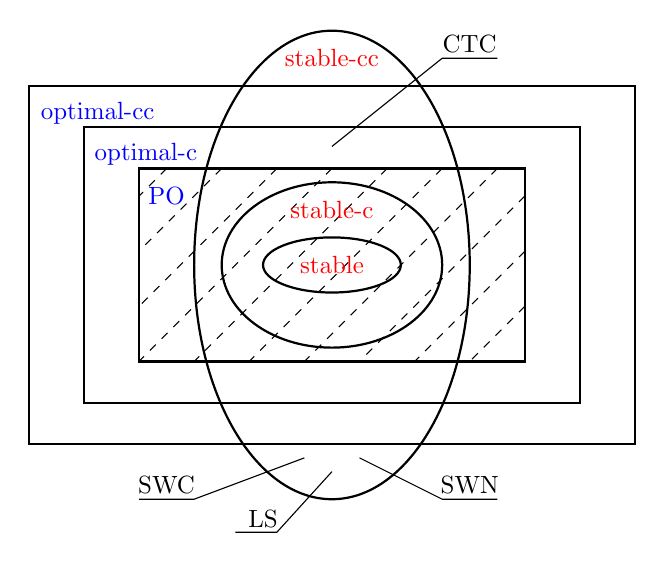
\begin{tikzpicture}[scale=0.35, sibling distance=5em,
  every node/.style = {scale=0.9, shape=circle, draw=none, align=center},
    outline/.style={draw=#1,thick,fill=#1!100}]
  every draw/.style = {scale=1}
  %pattern={north east lines}, 
  \draw[color=black,thick] (-1,2) rectangle (21,15);
  \draw[color=black,thick] (1,3.5) rectangle (19,13.5);
  \draw[draw=black, thick] (3,5) rectangle (17,12);
  \draw[dashed,color=black] (4,12) -- (3,11);
  \draw[dashed,color=black] (6,12) -- (3,9);
  \draw[dashed,color=black] (8,12) -- (3,7);
  \draw[dashed,color=black] (10,12) -- (3,5);
  \draw[dashed,color=black] (12,12) -- (5,5);
  \draw[dashed,color=black] (14,12) -- (7,5);
  \draw[dashed,color=black] (16,12) -- (9,5);
  \draw[dashed,color=black] (17,11) -- (11,5);
  \draw[dashed,color=black] (17,9) -- (13,5);
  \draw[dashed,color=black] (17,7) -- (15,5);
 
  \draw[color=black,thick] (10,8.5) ellipse (2.5 and 1);
  \draw[color=black,thick] (10,8.5) ellipse (4 and 3);
    % \draw[color=black,thick] (10,8.5) ellipse (4.95 and 4.95);
  \draw[color=black,thick] (10,8.5) ellipse (5 and 8.5);
  
  \node[color=blue] (node1) at (1.5,14) {optimal-cc};
  \node[color=blue] (node2) at (3.25,12.5) {optimal-c};
  \node[color=blue] (node3) at (4,11) {PO};
  \node[color=red] (node4) at (10,8.5) {stable};
  \node[color=red] (node5) at (10,10.5) {stable-c};
  % \node[color=red] (node7) at (10,12.5) {stable-strict-c};
  \node[rectangle,color=red] (node6) at (10,16) {stable-cc};
%  \filldraw[black] (12.25,1.25) circle (3pt) node[anchor=west]{SWN};
%  \filldraw[black] (7.8,1) circle (3pt) node[anchor=east]{SWC};
%  \filldraw[black] (10,0.5) circle (3pt) node[anchor=north]{LS};
%  \filldraw[black] (10,12.5) circle (3pt) node[anchor=west]{Our Mechanism};
  
%   \draw[color=black] (9,4) -- (12,-2) -- (18,-2);
%   \node[color=black] (node7) at (15,-1.5) {Our Mechanism};
  
  
  \draw[color=black] (9,1.5) -- (5,0) -- (3,0);
  \draw[color=black] (10,1) -- (8,-1.2) -- (6.5,-1.2);
  \draw[color=black] (11,1.5) -- (14,0) -- (16,0);
  \draw[color=black] (10,12.8) -- (14,16) -- (16,16);
  \node[rectangle,color=black] (node7) at (15,16.5) {CTC};
  \node[rectangle,color=black] (node8) at (4,0.5) {SWC};
  \node[rectangle,color=black] (node9) at (7.5,-0.7) {LS};
  \node[rectangle,color=black] (node10) at (15,0.5) {SWN};
  
\end{tikzpicture}
\caption{Venn diagram for optimality and stability notions. The shadowed area cannot coexist with IC and IR. }
\label{fig:Venn}
\end{figure}

%By definition, Pareto optimal implies optimal-c and further implies optimal-cc. Similarly, stable implies stable-c and further implies stable-cc. We also prove that both stable and stable-c imply Pareto optimal while there exists no implications between other versions of stability and optimality. Since Pareto optimal is not compatible with IC and IR, the theoretical boundaries for an incentive compatible diffusion matching mechanism are attaining stable-cc and optimal-c. We show that all existing mechanisms, SWN, SWC and LS~\cite{Leave_and_Share}, cannot satisfy any version of optimality. In this paper, we design a mechanism satisfying optimal-c and stable-cc, which reaches the theoretical boundaries for diffusion one-sided matching. 

%To begin with, we prove that if a mechanism is stable, it satisfies Pareto optimal.

By definition, Pareto optimality implies optimal-c and further implies optimal-cc. Similarly, stable implies stable-c and further implies stable-strict-c and stable-cc. The following theorems help us depict the relationship between optimal and stable properties.

\begin{theorem}
A mechanism $\pi$ is stable implies that $\pi$ is Pareto optimal.
\end{theorem}
\begin{proof}
For all type profiles $\theta$, if a stable mechanism $\pi$ is not Pareto optimal, there exists a group $T$ and $\pi'$ such that $\forall j\in T$, $\pi'_j(\theta) \succ_j \pi_j(\theta)$, and $\forall i\in N$, $\pi'_i(\theta) \succeq_i \pi_i(\theta)$. In this case, we can construct a group of agents $S$ starting from $T$, and consecutively add other agents so that $\forall i \in S$, $\pi'_i(\theta)\in H_S$. So, $S$ can deviate from the matching together which violates stable. Thus, $\pi$ is stable implies that $\pi$ is Pareto optimal.
\end{proof}

%We then prove that even stable-c, a weaker version of stability, implies Pareto optimal.
\begin{theorem}
A mechanism $\pi$ is stable-c implies that $\pi$ is Pareto optimal.
\end{theorem}
\begin{proof}
For all type profiles $\theta$, if $\pi$ is stable under connected components but fails Pareto optimal, there exists a group $T$ and $\pi'$ such that $\forall j\in T$, $\pi'_j(\theta) \succ_j \pi_j(\theta)$, and $\forall i\in N$, $\pi'_i(\theta) \succeq_i \pi_i(\theta)$. Since in diffusion one-sided matching, the unqualified agents always get their own items, agents in group $T$ must be the qualified agents. Given that all qualified agents is a connected component, they can deviate together to get $\pi'$ which violates stable under connected components. Thus, $\pi$ is stable-c implies that $\pi$ is Pareto optimal. 
\end{proof}

%Nevertheless, the implication between stability and Pareto optimality does not hold if we take another step to stable-cc.

% \begin{theorem}
% A mechanism $\pi$ is stable-strict-c implies that $\pi$ is optimal-c.
% \end{theorem}
% \begin{proof}
% For all type profiles $\theta$, if $\pi$ is stable-strict-c but it fails optimal-c, there exists a group of connected agents $T$ and $\pi'$ such that $\forall j\in T$, $\pi'_j(\theta) \succ_j \pi_j(\theta)$, and $\forall i\in N$, $\pi'_i(\theta) \succeq_i \pi_i(\theta)$. This violates stable-strict-c since all qualified agents form a connected component, and the strictly better off agents $T$ is a connected component. Thus, $\pi$ is stable-strict-c implies that $\pi$ is optimal-c.
% \end{proof}

% \begin{theorem}
% A mechanism $\pi$ is stable-strict-c cannot imply that $\pi$ is Pareto optimal.
% \end{theorem}
% \begin{proof}
% Consider the example given in Figure~\ref{fig:sta1}. Allocation $\pi$=($h_1,h_2,h_3$) satisfies stable-strict-c, but there exists another allocation $\pi'$=($h_3,h_2,h_1$) where agent 1 and 3 get better off, and agent 2 is not worse off. This means, $\pi$ is Pareto dominated by $\pi'$. Thus, $\pi$ is stable-strict-c cannot imply that $\pi$ is Pareto optimal.
% \end{proof}

% \begin{figure}[ht]
% \centering
% \begin{tikzpicture}[scale=0.22, sibling distance=5em,
%   every node/.style = {scale=0.8, shape=circle, draw, align=center},
%     outline/.style={draw=#1,thick,fill=#1!100}]
%   every draw/.style = {scale=1}
%   \node[] (node1) at (0,0) {1};
%   \node[] (node2) at (4,0) {2};
%   \node[] (node3) at (8,0) {3};
%   \draw[latex-latex] (node1)--(node2);
%   \draw[latex-latex] (node2)--(node3);
% \end{tikzpicture}
% \caption{Preferences are $h_3 \succ_1 h_1 \succ_1 h_2, \ \ \ h_1 \succ_2 h_2 \succ_2 h_3, \ \ \ h_1 \succ_3 h_3 \succ_3 h_2$. }
% \label{fig:sta1}
% \end{figure}

\begin{theorem}
A mechanism $\pi$ is stable-cc does not imply that $\pi$ is optimal-cc.
\end{theorem}
\begin{proof}
Consider the example given in Figure~\ref{fig:figure1}, allocation $\pi=(h_2,h_1,h_4,h_3)$ is stable under complete components. However, there exists another allocation $\pi'=(h_2,h_4,h_1,h_3)$ where \{2,3\} is a strictly better off group. This means the stable-cc mechanism $\pi$ fails to be optimal-cc.
\end{proof}

\begin{figure}[ht]
\centering
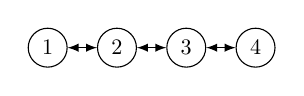
\begin{tikzpicture}[scale=0.22, sibling distance=5em,
  every node/.style = {scale=0.8, shape=circle, draw, align=center},
    outline/.style={draw=#1,thick,fill=#1!100}]
  every draw/.style = {scale=1}
  \node[] (node1) at (0,0) {1};
  \node[] (node2) at (4,0) {2};
  \node[] (node3) at (8,0) {3};
  \node[] (node4) at (12,0) {4};
  \draw[latex-latex] (node1)--(node2);
  \draw[latex-latex] (node2)--(node3);
  \draw[latex-latex] (node3)--(node4);
\end{tikzpicture}
\caption{Preferences are $h_3 \succ_1 h_2 \succ_1 h_1, \ \ \ h_4 \succ_2 h_1 \succ_2 h_2, \ \ \ h_1 \succ_3 h_4 \succ_3 h_3, \ \ \ h_2 \succ_4 h_3 \succ_4 h_4$. }
\label{fig:figure1}
\end{figure}

%Though both stable and stable-c imply Pareto optimal, the reverse implication does not stand. The next theorem states that Pareto optimal cannot imply stable-cc.

\begin{theorem}
A mechanism $\pi$ is Pareto optimal does not imply that $\pi$ is stable-cc. 
\end{theorem}
\begin{proof}
Consider the example given in Figure~\ref{fig:figure2}, allocation $\pi=(h_2,h_3,h_4,h_1)$ is Pareto optimal. But it fails stable under complete components because there exists another allocation $\pi'=(h_1,h_2,h_4,h_3)$ where \{3,4\} is a complete component, they deviate and swap among themselves for a better match compared to $\pi$. The existence of this subset of agents violates stable under complete components. Thus, Pareto optimal fails to imply stable-cc.
\end{proof}


\begin{figure}[ht]
\centering
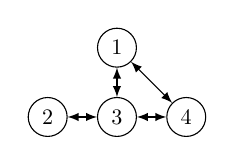
\begin{tikzpicture}[scale=0.22, sibling distance=5em,
  every node/.style = {scale=0.8, shape=circle, draw, align=center},
    outline/.style={draw=#1,thick,fill=#1!100}]
  every draw/.style = {scale=1}
%   \node[] (node1) at (6,3) {1};
  \node[] (node1) at (4,4) {1};
  \node[] (node2) at (0,0) {2};
  \node[] (node3) at (4,0) {3};
  \node[] (node4) at (8,0) {4};
  \draw[latex-latex] (node1)--(node3);
  \draw[latex-latex] (node1)--(node4);
  \draw[latex-latex] (node2)--(node3);
  \draw[latex-latex] (node3)--(node4);
\end{tikzpicture}
\caption{Preferences are $h_2 \succ_1 h_3 \succ_1 h_1, \ \ \ h_3 \succ_2 h_2, \ \ \ h_2 \succ_3 h_4 \succ_3 h_3, \ \ \ h_3 \succ_4 h_1 \succ_4 h_4$. }
\label{fig:figure2}
\end{figure}


We can see that the theoretical boundary for diffusion one-sided matching is attaining stable-cc and optimal-c. However, this boundary is not attainable by any of the mechanisms proposed in the literature so far.
\begin{theorem}
Swap With Children, Leave and Share, and Swap With Neighbor presented by \citeauthor{DBLP:conf/atal/KawasakiWTY21} and \citeauthor{Leave_and_Share} cannot satisfy optimal-c.
\end{theorem}
\begin{proof}
In the example given in Figure~\ref{fig:figure1}, the allocations given by SWC, LS and SWN are identical, which is $\pi=(h_2,h_1,h_4,h_3)$. There exists an optimal-c allocation $\pi'=(h_2,h_4,h_1,h_3)$ that dominates $\pi$. Thus, these mechanisms fail optimal-c.
\end{proof}

In the next section, we present a mechanism called Connected Trading Cycles (CTC), which allow agent 1 and 3, agent 2 and 4 swap with each other in Figure~\ref{fig:figure1}. We also prove that CTC satisfies optimal-c, which means it dominates the other three mechanisms and reach the theoretical boundary.

%%%%%%%%%%%%%%%%%%%%%%%%%%%%%%%%%%%%%%%%%%%%%%%%%%%%%%%%%%%%%%%%%%%%%%%%
\section{Connected Trading Cycles}
In this section, we present our mechanism called Connected Trading Cycles (CTC) which takes both the trading cycles and agents' connections into concerns. CTC can satisfy IC, optimal-c and stable-cc, which is the theoretical boundary of the network setting. First of all, several definitions are declared to simplify the description of our mechanism.

\begin{definition}
Given a reported type profile $\theta'$, we generate a directed graph $F(\theta')$, in which each qualified agent has exactly one out-degree pointing to any qualified agent in $G(\theta')$. The pointing from each agent $i$ to $j$ ($i,j$ can be the same agent) means $j$ is a qualified agent and $h_j$ is the smallest ranked item in $\succ_i'$. We name the graph as the favorite pointing graph for $\theta'$. 
\end{definition}

There is at least one cycle in $F(\theta')$ and we should clarify whether the cycles can get traded or not. We classify the cycles into three categories, independent connected-cycles, dependent connected-cycles and unconnected-cycles, defined as follows. In this paper, we use connected-cycle to represent either dependent connected-cycle or independent connected-cycle for simplicity. 

\begin{definition}
Given a favorite pointing graph $F(\theta')$ and a node sequence $(c_1,c_2,...,c_m)$, for simplicity we use $C_i$ to represent the node sequence in which $i=c_m$. If there exists an edge $\langle c_{j},c_{j+1}\rangle$ for any $c_j \in C_i, c_j \neq c_m$ and $\langle c_m,c_1\rangle $, then there is a cycle involving $C_i$ in $F(\theta')$, we denote the cycle by $C_i$.

\end{definition}

\begin{enumerate}
    \item[a.] $C_i$ is an \textbf{independent connected-cycle} in $F(\theta')$ if all agents in $C_i$ can form a connected component in $G(\theta')$.
    \item[b.] $C_i$ is a \textbf{dependent connected-cycle} if there exists a cycle set $\mathbb{C}=\{C_i, C_j, \dots \}$ in $F(\theta')$ and all agents in $\mathbb{C}$ can form a connected component in $G(\theta')$, $\forall \mathbb{C'} \subsetneq \mathbb{C}$, all agents in $\mathbb{C'}$ cannot form a connected component in $G(\theta')$.

    \item[c.]All cycles other than a. and b. are \textbf{unconnected-cycles}.
    
\end{enumerate}
%figure used to be here
We illustrate the three types of cycles in Figure~\ref{fig:cycles}. As shown in sub-figure (a), $C_4 = (1,3,2,4)$ is an independent connected-cycle. In sub-figure (b), $C_3 = (1,3)$ and $C_4 = (2,4)$ are two dependent connected-cycles. In sub-figure (c), $C_3 = (2,3)$ is an independent connected-cycle, and $C_4 = (1,4)$ is an unconnected-cycle.
\begin{figure*}[ht]
\centering

\subfigure[]{
\centering
\begin{minipage}[t]{0.3\linewidth}
\centering
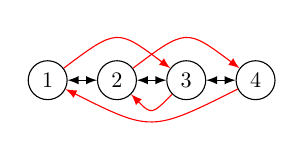
\begin{tikzpicture}[scale=0.22, sibling distance=0em,
  every node/.style = {scale=0.8, shape=circle, draw, align=center},
    outline/.style={draw=#1,thick,fill=#1!100}]
  every draw/.style = {scale=2}
  \node[] (node1) at (0,0) {1};
  \node[] (node2) at (4,0) {2};
  \node[] (node3) at (8,0) {3};
  \node[] (node4) at (12,0) {4};
  \draw[latex-latex] (node1)--(node2);
  \draw[latex-latex] (node2)--(node3);
  \draw[latex-latex] (node3)--(node4);
  

  \draw[-latex,red] (node1).. controls(4,3) ..(node3);
  \draw[-latex,red] (node3).. controls(6,-2) ..(node2);
  \draw[-latex,red] (node2).. controls(8,3) ..(node4);
  \draw[-latex,red] (node4).. controls(6,-3) ..(node1);
\end{tikzpicture}
%-{Latex[length=2mm]},blue,line width=1.2pt
%-latex,red,line width=0.3pt
\end{minipage}
}
\subfigure[]{
\centering
\begin{minipage}[t]{0.3\linewidth}
\centering
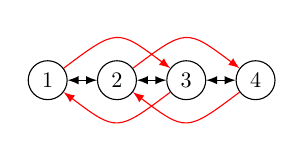
\begin{tikzpicture}[scale=0.22, sibling distance=0em,
  every node/.style = {scale=0.8, shape=circle, draw, align=center},
    outline/.style={draw=#1,thick,fill=#1!100}]
  every draw/.style = {scale=2}
    \node[] (node1) at (0,0) {1};
  \node[] (node2) at (4,0) {2};
  \node[] (node3) at (8,0) {3};
  \node[] (node4) at (12,0) {4};
  \draw[latex-latex] (node1)--(node2);
  \draw[latex-latex] (node2)--(node3);
  \draw[latex-latex] (node3)--(node4);
  

  \draw[-latex,red] (node1).. controls(4,3) ..(node3);
  \draw[-latex,red] (node3).. controls(4,-3) ..(node1);
  \draw[-latex,red] (node2).. controls(8,3) ..(node4);
  \draw[-latex,red] (node4).. controls(8,-3) ..(node2);
\end{tikzpicture}


\end{minipage}
}
\subfigure[]{
\centering
\begin{minipage}[t]{0.3\linewidth}
\centering
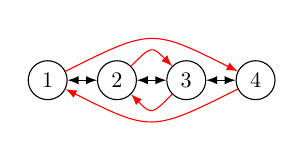
\begin{tikzpicture}[scale=0.22, sibling distance=0em,
  every node/.style = {scale=0.8, shape=circle, draw, align=center},
    outline/.style={draw=#1,thick,fill=#1!100}]
  every draw/.style = {scale=2}
  
   \node[] (node1) at (0,0) {1};
  \node[] (node2) at (4,0) {2};
  \node[] (node3) at (8,0) {3};
  \node[] (node4) at (12,0) {4};
  \draw[latex-latex] (node1)--(node2);
  \draw[latex-latex] (node2)--(node3);
  \draw[latex-latex] (node3)--(node4);
  

  \draw[-latex,red] (node1).. controls(6,3) ..(node4);
  \draw[-latex,red] (node4).. controls(6,-3) ..(node1);
  \draw[-latex,red] (node2).. controls(6,2) ..(node3);
  \draw[-latex,red] (node3).. controls(6,-2) ..(node2);

\end{tikzpicture}


\end{minipage}
}

\caption{Examples of independent connected-cycles, dependent connected-cycles and unconnected-cycles. Double arrows represent agents' connections in $G(\theta')$, and red single arrows represent their favorite pointing.}
\label{fig:cycles}
\end{figure*}


The heart of our mechanism is to find connected-cycles in the favorite pointing graph $F(\theta')$ and let them get traded. Inspired by the sharing idea first proposed by \citeauthor{Leave_and_Share}, we first match the connected-cycles in the favorite pointing graph, and share their neighbors to construct more connectivity among agents. This will not cause incompatibility with IC because agents who get their favorite item have no incentives to misreport, nor do they care about the rest of the market.

Unfortunately, not all agents can get their most preferred item, some have to switch their pointing in $F(\theta')$ to a less preferred one. So, we define a next favorite function to adjust $F(\theta')$ based on agents' preferences.

\begin{definition}
Given a reported type profile $\theta'$ and a favorite pointing graph $F(\theta')$, we have $\succ_i^{next}(F(\theta'))=j, j \in Q(\theta')$, if $j$ is the qualified agent who owns $i$'s next favorite item.
\end{definition}

Since our mechanism involves preference switching, we need a strategy-proof order, defined upon agent's shortest length to the initial players, to decide which agent should switch her preference under certain circumstances.

\begin{definition}
An order of agents is a one-to-one function $\mathcal {O}:\mathbb {N}^{+}\to N$, where agent $\mathcal {O}(i)$ is the $i^{th}$ agent in the order. Agents in $\mathcal{O}$ are sorted in ascending order by the length of the shortest path from agent set $N_0$ to them. Especially, for any agent $i \in N_0$, its shortest path length is $0$. When multiple agents have the same length of the shortest path, we use a random tie-breaking. 
\end{definition}



Now we are ready to introduce our mechanism.

\begin{framed}
\noindent\textbf{Connected Trading Cycles}

Given a reported type profile $\theta'$, construct the favorite pointing graph $F(\theta')$. Initiate a settled agent set $V=\emptyset$.

% \begin{enumerate}
    % \item[1.] While there exists a group of agents $S$, $\forall i\in S, \succ^{N\setminus V}_i(1)\in H_S$, and $\forall i,j \in S, \succ^{N\setminus V}_i(1)\neq\succ^{N\setminus V}_j(1)$, and $S$ or $S\cup V$ is a connected component in $G(\theta')$. Add $S$ into $V$. Connected the neighbors of all agents in $S$ as neighbors of each other. That is, update $\cup_{i\in S}r_i$ as a complete component.

    % \item[1.] While there exists a connected-cycle $C$ in $F(\theta')$, add all agents involved in $C$ into $V$, and connect their neighbors with each other in $G(\theta')$. While there exists an edge $\langle p,q\rangle $ in $F(\theta')$ that satisfies $p \in N \setminus V, q \in V$, change $\langle p,q\rangle $ to $\langle p,\succ_p^{next}(F(\theta'))\rangle $.

    % \item[2.] 
    Executing the following steps until $V=N$
\begin{enumerate}

    \item[a.] Find the agent $i \in N \setminus V$ with 0 in-degree in $F(\theta')$ who has the minimum order. If there is no 0 in-degree agent, find the agent $i \in N \setminus V$ with the minimum order.
    
    \item[b.]Detect a path $P_{p_1}=(p_1,\dots,p_k,\dots,p_m)$ in $F(\theta')$ starting from $p_1$ that satisfies there exists an edge $\langle p_{j},p_{j+1}\rangle $ for any $p_j \in P_i, p_j \neq p_m$, and $\langle p_m,p_k\rangle $. Especially, $C_{p_m}=(p_k,\dots,p_m)$ is a cycle in $F(\theta')$.
    \begin{enumerate}
    
    \item[i] If $C_{p_m}$ is an independent connected-cycle or a dependent connected-cycle, add all agents in $C_{p_m}$ to settled agent set $V$.
    
    \item[ii] If $C_{p_m}$ is an unconnected-cycle, reversely track $P_{p1}$ from $p_m$ to $p_1$, find the first $p_{l-1}$ who points to an agent $p_l$ and no connected component containing $p_{l-1}$ and $p_l$ in $G(\theta')$ is a subset of $C_{p_m}$. If $l=m$ and any path from $p_{k-1}$ to $p_k$ passes through $p_m$, change edge$\langle p_{k-1},p_{k}\rangle $ to $\langle p_{k-1},\succ_{p_{k-1}}^{next}(F(\theta'))\rangle $. Otherwise, change the edge $\langle p_{l},p_{l'}\rangle $ to $\langle p_{l},\succ_{p_{l}^{next}}(F(\theta'))\rangle $.
    
    \end{enumerate}

    \item[c.] While there exists an edge $\langle p,q\rangle $ in $F(\theta')$ that satisfies $p \in N \setminus V, q \in V$, change $\langle p,q\rangle $ to $\langle p,\succ_p^{next}(F(\theta'))\rangle $
\end{enumerate}
% \end{enumerate}




\end{framed}

\begin{figure*}[t]
\centering

\begin{minipage}[]{0.45\linewidth}
\centering

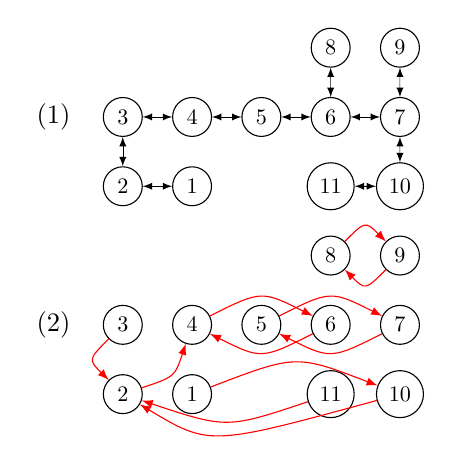
\begin{tikzpicture}[scale=0.22, sibling distance=0em,
  every node/.style = {scale=0.8, shape=circle, draw, align=center},
    outline/.style={draw=#1,thick,fill=#1!100}]
  every draw/.style = {scale=2}
  \node[] (node1) at (4,-4) {1};
  \node[] (node2) at (0,-4) {2};
  \node[] (node3) at (0,0) {3};
  \node[] (node4) at (4,0) {4};
  \node[] (node5) at (8,0) {5};
  \node[] (node6) at (12,0) {6};
  \node[] (node7) at (16,0) {7};
  \node[] (node8) at (12,4) {8};
  \node[] (node9) at (16,4) {9};
  \node[] (node10) at (16,-4) {10};
  \node[] (node11) at (12,-4) {11};
  \draw[latex-latex,very thin] (node1)--(node2);
  \draw[latex-latex,very thin] (node2)--(node3);
  \draw[latex-latex,very thin] (node3)--(node4);
  \draw[latex-latex,very thin] (node4)--(node5);
  \draw[latex-latex,very thin] (node5)--(node6);
  \draw[latex-latex,very thin] (node6)--(node7);
  \draw[latex-latex,very thin] (node6)--(node8);
  \draw[latex-latex,very thin] (node7)--(node9);
  \draw[latex-latex,very thin] (node7)--(node10);
  \draw[latex-latex,very thin] (node10)--(node11);
  
  %\draw[dashed,very thin] (-4,-6)--(20,-6);
  %\draw[dashed,very thin] (-4,6)--(20,6);
  %\draw[dashed,very thin] (-4,-20)--(20,-20);
  %\draw[dashed,very thin] (-4,6)--(-4,-20);
  %\draw[dashed,very thin] (20,-20)--(20,6);
  
  
  \node[scale=1.2,draw=none,rectangle] (node20) at (-4,0) {(1)};
  \node[scale=1.2,draw=none,rectangle] (node21) at (-4,-12) {(2)};
  
  \node[] (node01) at (4,-16) {1};
  \node[] (node02) at (0,-16) {2};
  \node[] (node03) at (0,-12) {3};
  \node[] (node04) at (4,-12) {4};
  \node[] (node05) at (8,-12) {5};
  \node[] (node06) at (12,-12) {6};
  \node[] (node07) at (16,-12) {7};
  \node[] (node08) at (12,-8) {8};
  \node[] (node09) at (16,-8) {9};
  \node[] (node010) at (16,-16) {10};
  \node[] (node011) at (12,-16) {11};
  
  \draw[-latex,red] (node01).. controls(10,-13.7) ..(node010);
  \draw[-latex,red] (node02).. controls(3,-15) ..(node04);
  \draw[-latex,red] (node03).. controls(-2,-14) ..(node02);
  \draw[-latex,red] (node04).. controls(8,-10) ..(node06);
  \draw[-latex,red] (node05).. controls(12,-10) ..(node07);
  \draw[-latex,red] (node06).. controls(8,-14) ..(node04);
  \draw[-latex,red] (node07).. controls(12,-14) ..(node05);
  \draw[-latex,red] (node08).. controls(14,-6) ..(node09);
  \draw[-latex,red] (node09).. controls(14,-10) ..(node08);
  \draw[-latex,red] (node010).. controls(5,-19) ..(node02);
  \draw[-latex,red] (node011).. controls(6,-18) ..(node02);
  
\end{tikzpicture}


\end{minipage}
\begin{minipage}[t]{0.35\linewidth}
\centering

\begin{tabular}{|c|l|l|l|}
\hline
i & $\succ_i$  & $r_i$ & $\pi_i$ \\ \hline
1 & $h_{10} \succ h_2 \succ \cdots$ & 2 & $h_2$ \\ \hline
2 & $h_4 \succ h_1  \succ \cdots$ & 1,3 & $h_1$\\ \hline
3 & $h_2 \succ h_3  \succ \cdots$ & 2,4 & $h_3$\\ \hline
4 & $h_6 \succ \cdots $ & 3,5 & $h_6$\\ \hline
5 & $h_7 \succ \cdots$ & 4,6 & $h_7$\\ \hline
6 & $h_4 \succ \cdots$ & 5,7,8 & $h_4$\\ \hline
7 & $h_5 \succ \cdots$ & 6,9,10 & $h_5$\\ \hline
8 & $h_9 \succ h_8 \succ \cdots$ & 6 & $h_8$\\ \hline
9 & $h_8 \succ h_9 \succ \cdots$ & 7 & $h_9$\\ \hline
10 & $h_2 \succ h_{11} \succ \cdots$ & 7,11 & $h_{11}$\\ \hline
11 & $h_2 \succ h_{10} \succ \cdots$ & 10 & $h_{10}$\\ \hline
\end{tabular}

\end{minipage}
\caption{Sub-figure (1) represents the $G(\theta')$. Sub-figure (2) is the favorite pointing graph $F(\theta')$. The table presents the preference, neighbor set, and the allocation given by CTC for each agent. }
\label{fig:pref_table}
\end{figure*}

In our mechanism, the allocation relies on the cycles in the favorite pointing graph. These cycles ensure optimality, so agents will truthfully report their preferences. We further classify the cycles by social connections and protect the connected-cycles while break the unconnected-cycles. We allow the connected-cycles to form because their connectivity is only determined by agents in the cycles and cannot be influenced by others. It is natural for the independent connected-cycle since the cycle itself is formed by a connected component. For the dependent connected-cycle, we require that no subset of the cycle set be a connected component. Namely, all agents in the cycle set rely on each other to form connected-cycle and get traded, so they share the same interest. This prevents agents from misreporting to form connected-cycles for their own good using the already formed cycles. To sum up, these two types of connected-cycles target at allowing cycles in the favorite pointing graph as much as possible. As for the unconnected-cycles, to maintain optimality, we try to sustain the favorite pointing along the cycles to the greatest extent. We only let those who cannot connect to her pointing with the help of the cycle switch pointing (as in b.ii).

%\textcolor{red}{For the similar reason, we require that no one in the connected component will prevent others joining in the connected component. By doing so, those agents can forcefully form a dependent connected-cycle which will harm other agents inside the connected component.}

We present a detailed example to illustrate our mechanism. The initial agent set is $N_0=\{ 1 \}$. The order is $\mathcal{O}=(1,2,3,4,5,6,7,8,9,$ $10,11)$. The social network, type profiles, and allocation are presented in Figure~\ref{fig:pref_table}. The following steps match the sub-figures in Figure~\ref{fig:run_example}.




\begin{figure*}[t]
\centering

% \subfigure[]{
% \centering
% \begin{minipage}[t]{0.3\linewidth}
% \centering
% \begin{tikzpicture}[scale=0.22, sibling distance=0em,
%   every node/.style = {scale=0.7, shape=circle, draw, align=center},
%     outline/.style={draw=#1,thick,fill=#1!100}]
%   every draw/.style = {scale=2}
%   \node[line width=1pt] (node1) at (4,-4) {1};
%   \node[] (node2) at (0,-4) {2};
%   \node[] (node3) at (0,0) {3};
%   \node[dashed,fill=black!10] (node4) at (4,0) {4};
%   \node[dashed,fill=black!10] (node5) at (8,0) {5};
%   \node[dashed,fill=black!10] (node6) at (12,0) {6};
%   \node[dashed,fill=black!10] (node7) at (16,0) {7};
%   \node[] (node8) at (12,4) {8};
%   \node[] (node9) at (16,4) {9};
%   \node[] (node10) at (16,-4) {10};
%   \node[] (node11) at (12,-4) {11};
%   \draw[very thin] (node1)--(node2);
%   \draw[very thin] (node2)--(node3);
%   \draw[very thin] (node3)--(node4);
%   \draw[very thin] (node4)--(node5);
%   \draw[very thin] (node5)--(node6);
%   \draw[very thin] (node6)--(node7);
%   \draw[very thin] (node6)--(node8);
%   \draw[very thin] (node7)--(node9);
%   \draw[very thin] (node7)--(node10);
%   \draw[very thin] (node10)--(node11);
  
%   \draw[-latex,red] (node1).. controls(10,-1.7) ..(node10);
%   \draw[-latex,red] (node2).. controls(3,-3) ..(node4);
%   \draw[-latex,red] (node3).. controls(-2,-2) ..(node2);
%   \draw[-latex,red] (node4).. controls(8,2) ..(node6);
%   \draw[-latex,red] (node5).. controls(12,2) ..(node7);
%   \draw[-latex,red] (node6).. controls(8,-2) ..(node4);
%   \draw[-latex,red] (node7).. controls(12,-2) ..(node5);
%   \draw[-latex,red] (node8).. controls(14,6) ..(node9);
%   \draw[-latex,red] (node9).. controls(14,2) ..(node8);
%   \draw[-latex,red] (node10).. controls(5,-7) ..(node2);
%   \draw[-latex,red] (node11).. controls(6,-6) ..(node2);
% %  \draw[-latex,blue,dashed] (node1).. controls(2,-2) ..(node2);
% %  \draw[-latex,blue,dashed] (node2).. controls(2,-2) ..(node1);
% %  \draw[-latex,red,dashed] (node3).. controls(-1,2) and (1,2) ..(node3);
% %  \draw[-latex,red,dashed] (node10).. controls(14,-2) ..(node11);
% %  \draw[-latex,red,dashed] (node11).. controls(14,-6) ..(node10);
% \end{tikzpicture}
% %-{Latex[length=2mm]},blue,line width=1.2pt
% %-latex,red,line width=0.3pt

% \end{minipage}
% }
% \subfigure[]{
% \centering
% \begin{minipage}[t]{0.3\linewidth}
% \centering
% \begin{tikzpicture}[scale=0.22, sibling distance=0em,
%   every node/.style = {scale=0.7, shape=circle, draw, align=center},
%     outline/.style={draw=#1,thick,fill=#1!100}]
%   every draw/.style = {scale=2}
%   \node[line width=1pt] (node1) at (4,-4) {1};
%   \node[] (node2) at (0,-4) {2};
%   \node[] (node3) at (0,0) {3};
%   \node[dashed,fill=black!10] (node4) at (4,0) {4};
%   \node[dashed,fill=black!10] (node5) at (8,0) {5};
%   \node[dashed,fill=black!10] (node6) at (12,0) {6};
%   \node[dashed,fill=black!10] (node7) at (16,0) {7};
%   \node[dashed,fill=black!10] (node8) at (12,4) {8};
%   \node[dashed,fill=black!10] (node9) at (16,4) {9};
%   \node[] (node10) at (16,-4) {10};
%   \node[] (node11) at (12,-4) {11};
%   \draw[very thin] (node1)--(node2);
%   \draw[very thin] (node2)--(node3);
%   \draw[very thin] (node3)--(node4);
%   \draw[very thin] (node4)--(node5);
%   \draw[very thin] (node5)--(node6);
%   \draw[very thin] (node6)--(node7);
%   \draw[very thin] (node6)--(node8);
%   \draw[very thin,dashed] (node3)--(node8);
%   \draw[very thin,dashed] (node3)--(node9);
%   \draw[very thin,dashed] (node3)--(node10);
%   \draw[very thin,dashed] (node8)--(node9);
%   \draw[very thin,dashed] (node8)--(node10);
%   \draw[very thin,dashed] (node9)--(node10);
%   \draw[very thin] (node7)--(node9);
%   \draw[very thin] (node7)--(node10);
%   \draw[very thin] (node10)--(node11);
  
%   \draw[-latex,red] (node1).. controls(10,-1.7) ..(node10);
%   \draw[-latex,red] (node2).. controls(3,-3) ..(node4);
%   \draw[-latex,red] (node3).. controls(-2,-2) ..(node2);
%   \draw[-latex,red] (node4).. controls(8,2) ..(node6);
%   \draw[-latex,red] (node5).. controls(12,2) ..(node7);
%   \draw[-latex,red] (node6).. controls(8,-2) ..(node4);
%   \draw[-latex,red] (node7).. controls(12,-2) ..(node5);
%   \draw[-latex,red] (node8).. controls(14,6) ..(node9);
%   \draw[-latex,red] (node9).. controls(14,2) ..(node8);
%   \draw[-latex,red] (node10).. controls(5,-7) ..(node2);
%   \draw[-latex,red] (node11).. controls(6,-6) ..(node2);
% %  \draw[-latex,blue,dashed] (node1).. controls(2,-2) ..(node2);
% %  \draw[-latex,blue,dashed] (node2).. controls(2,-2) ..(node1);
% %  \draw[-latex,red,dashed] (node3).. controls(-1,2) and (1,2) ..(node3);
% %  \draw[-latex,red,dashed] (node10).. controls(14,-2) ..(node11);
% %  \draw[-latex,red,dashed] (node11).. controls(14,-6) ..(node10);
% \end{tikzpicture}
% %-{Latex[length=2mm]},blue,line width=1.2pt
% %-latex,red,line width=0.3pt

% \end{minipage}
% }

\subfigure[]{
\centering
\begin{minipage}[t]{0.3\linewidth}
\centering
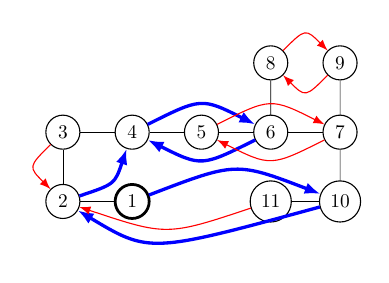
\begin{tikzpicture}[scale=0.22, sibling distance=0em,
  every node/.style = {scale=0.7, shape=circle, draw, align=center},
    outline/.style={draw=#1,thick,fill=#1!100}]
  every draw/.style = {scale=2}
  \node[line width=1pt] (node1) at (4,-4) {1};
  \node[] (node2) at (0,-4) {2};
  \node[] (node3) at (0,0) {3};
  \node[] (node4) at (4,0) {4};
  \node[] (node5) at (8,0) {5};
  \node[] (node6) at (12,0) {6};
  \node[] (node7) at (16,0) {7};
  \node[] (node8) at (12,4) {8};
  \node[] (node9) at (16,4) {9};
  \node[] (node10) at (16,-4) {10};
  \node[] (node11) at (12,-4) {11};
  \draw[very thin] (node1)--(node2);
  \draw[very thin] (node2)--(node3);
  \draw[very thin] (node3)--(node4);
  \draw[very thin] (node4)--(node5);
  \draw[very thin] (node5)--(node6);
  \draw[very thin] (node6)--(node7);
  \draw[very thin] (node6)--(node8);
  \draw[very thin] (node7)--(node9);
  \draw[very thin] (node7)--(node10);
  \draw[very thin] (node10)--(node11);
  
  \draw[-{Latex[length=2mm]},blue,very thick] (node1).. controls(10,-1.7) ..(node10);
  \draw[-{Latex[length=2mm]},blue,very thick] (node2).. controls(3,-3) ..(node4);
  \draw[-latex,red] (node3).. controls(-2,-2) ..(node2);
  \draw[-{Latex[length=2mm]},blue,very thick] (node4).. controls(8,2) ..(node6);
  \draw[-latex,red] (node5).. controls(12,2) ..(node7);
  \draw[-{Latex[length=2mm]},blue,very thick] (node6).. controls(8,-2) ..(node4);
  \draw[-latex,red] (node7).. controls(12,-2) ..(node5);
  \draw[-latex,red] (node8).. controls(14,6) ..(node9);
  \draw[-latex,red] (node9).. controls(14,2) ..(node8);
  \draw[-{Latex[length=2mm]},blue,very thick] (node10).. controls(5,-7) ..(node2);
  \draw[-latex,red] (node11).. controls(6,-6) ..(node2);
%  \draw[-latex,blue,dashed] (node1).. controls(2,-2) ..(node2);
%  \draw[-latex,blue,dashed] (node2).. controls(2,-2) ..(node1);
%  \draw[-latex,red,dashed] (node3).. controls(-1,2) and (1,2) ..(node3);
%  \draw[-latex,red,dashed] (node10).. controls(14,-2) ..(node11);
%  \draw[-latex,red,dashed] (node11).. controls(14,-6) ..(node10);
\end{tikzpicture}
%-{Latex[length=2mm]},blue,line width=1.2pt
%-latex,red,line width=0.3pt

\end{minipage}
}
\subfigure[]{
\centering
\begin{minipage}[t]{0.3\linewidth}
\centering
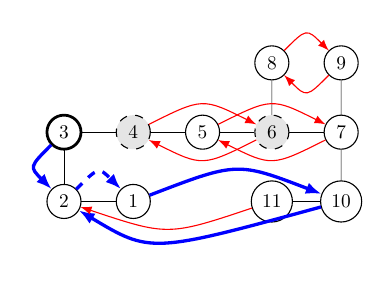
\begin{tikzpicture}[scale=0.22, sibling distance=0em,
  every node/.style = {scale=0.7, shape=circle, draw, align=center},
    outline/.style={draw=#1,thick,fill=#1!100}]
  every draw/.style = {scale=2}
  \node[] (node1) at (4,-4) {1};
  \node[] (node2) at (0,-4) {2};
  \node[line width=1pt] (node3) at (0,0) {3};
  \node[dashed, fill=black!10] (node4) at (4,0) {4};
  \node[] (node5) at (8,0) {5};
  \node[dashed, fill=black!10] (node6) at (12,0) {6};
  \node[] (node7) at (16,0) {7};
  \node[] (node8) at (12,4) {8};
  \node[] (node9) at (16,4) {9};
  \node[] (node10) at (16,-4) {10};
  \node[] (node11) at (12,-4) {11};
  \draw[very thin] (node1)--(node2);
  \draw[very thin] (node2)--(node3);
  \draw[very thin] (node3)--(node4);
  \draw[very thin] (node4)--(node5);
  \draw[very thin] (node5)--(node6);
  \draw[very thin] (node6)--(node7);
  \draw[very thin] (node6)--(node8);
  \draw[very thin] (node7)--(node9);
  \draw[very thin] (node7)--(node10);
  \draw[very thin] (node10)--(node11);
  
  \draw[-{Latex[length=2mm]},blue,very thick] (node1).. controls(10,-1.7) ..(node10);
%  \draw[-latex,red] (node2).. controls(3,-3) ..(node4);
  \draw[-{Latex[length=2mm]},blue,very thick] (node3).. controls(-2,-2) ..(node2);
  \draw[-latex,red] (node4).. controls(8,2) ..(node6);
  \draw[-latex,red] (node5).. controls(12,2) ..(node7);
  \draw[-latex,red] (node6).. controls(8,-2) ..(node4);
  \draw[-latex,red] (node7).. controls(12,-2) ..(node5);
  \draw[-latex,red] (node8).. controls(14,6) ..(node9);
  \draw[-latex,red] (node9).. controls(14,2) ..(node8);
  \draw[-{Latex[length=2mm]},blue,very thick] (node10).. controls(5,-7) ..(node2);
  \draw[-latex,red] (node11).. controls(6,-6) ..(node2);
%  \draw[-latex,blue,dashed] (node1).. controls(2,-2) ..(node2);
  \draw[-{Latex[length=2mm]},blue,very thick, dashed] (node2).. controls(2,-2) ..(node1);
%  \draw[-latex,red,dashed] (node3).. controls(-1,2) and (1,2) ..(node3);
%  \draw[-latex,red,dashed] (node10).. controls(14,-2) ..(node11);
%  \draw[-latex,red,dashed] (node11).. controls(14,-6) ..(node10);
\end{tikzpicture}


\end{minipage}
}
\subfigure[]{
\centering
\begin{minipage}[t]{0.3\linewidth}
\centering
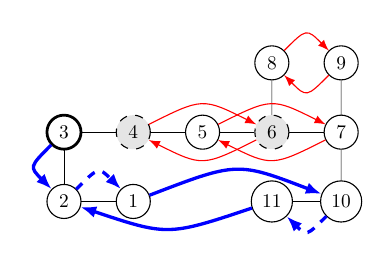
\begin{tikzpicture}[scale=0.22, sibling distance=0em,
  every node/.style = {scale=0.7, shape=circle, draw, align=center},
    outline/.style={draw=#1,thick,fill=#1!100}]
  every draw/.style = {scale=2}
  
  \node[] (node1) at (4,-4) {1};
  \node[] (node2) at (0,-4) {2};
  \node[line width=1pt] (node3) at (0,0) {3};
  \node[dashed, fill=black!10] (node4) at (4,0) {4};
  \node[] (node5) at (8,0) {5};
  \node[dashed, fill=black!10] (node6) at (12,0) {6};
  \node[] (node7) at (16,0) {7};
  \node[] (node8) at (12,4) {8};
  \node[] (node9) at (16,4) {9};
  \node[] (node10) at (16,-4) {10};
  \node[] (node11) at (12,-4) {11};
  \draw[very thin] (node1)--(node2);
  \draw[very thin] (node2)--(node3);
  \draw[very thin] (node3)--(node4);
  \draw[very thin] (node4)--(node5);
  \draw[very thin] (node5)--(node6);
  \draw[very thin] (node6)--(node7);
  \draw[very thin] (node6)--(node8);
  \draw[very thin] (node7)--(node9);
  \draw[very thin] (node7)--(node10);
  \draw[very thin] (node10)--(node11);
  
  \draw[-{Latex[length=2mm]},blue,very thick] (node1).. controls(10,-1.7) ..(node10);
%  \draw[-latex,red] (node2).. controls(3,-3) ..(node4);
  \draw[-{Latex[length=2mm]},blue,very thick] (node3).. controls(-2,-2) ..(node2);
  \draw[-latex,red] (node4).. controls(8,2) ..(node6);
  \draw[-latex,red] (node5).. controls(12,2) ..(node7);
  \draw[-latex,red] (node6).. controls(8,-2) ..(node4);
  \draw[-latex,red] (node7).. controls(12,-2) ..(node5);
  \draw[-latex,red] (node8).. controls(14,6) ..(node9);
  \draw[-latex,red] (node9).. controls(14,2) ..(node8);
%  \draw[-latex,red] (node10).. controls(8,-6) ..(node2);
  \draw[-{Latex[length=2mm]},blue,very thick] (node11).. controls(6,-6) ..(node2);
%  \draw[-latex,red,dashed] (node1).. controls(2,-2) ..(node2);
  \draw[-{Latex[length=2mm]},blue,very thick,dashed] (node2).. controls(2,-2) ..(node1);
%  \draw[-latex,red,dashed] (node3).. controls(-1,2) and (1,2) ..(node3);
  \draw[-{Latex[length=2mm]},blue,very thick,dashed] (node10).. controls(14,-6) ..(node11);
%  \draw[-latex,red,dashed] (node11).. controls(14,-6) ..(node10);

\end{tikzpicture}


\end{minipage}
}
\medskip
\subfigure[]{
\centering
\begin{minipage}[t]{0.3\linewidth}
\centering
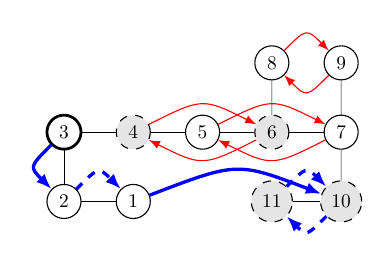
\begin{tikzpicture}[scale=0.22, sibling distance=0em,
  every node/.style = {scale=0.7, shape=circle, draw, align=center},
    outline/.style={draw=#1,thick,fill=#1!100}]
  every draw/.style = {scale=2}
  
  \node[] (node1) at (4,-4) {1};
  \node[] (node2) at (0,-4) {2};
  \node[line width=1pt] (node3) at (0,0) {3};
  \node[dashed, fill=black!10] (node4) at (4,0) {4};
  \node[] (node5) at (8,0) {5};
  \node[dashed, fill=black!10] (node6) at (12,0) {6};
  \node[] (node7) at (16,0) {7};
  \node[] (node8) at (12,4) {8};
  \node[] (node9) at (16,4) {9};
  \node[dashed, fill=black!10] (node10) at (16,-4) {10};
  \node[dashed, fill=black!10] (node11) at (12,-4) {11};
  \draw[very thin] (node1)--(node2);
  \draw[very thin] (node2)--(node3);
  \draw[very thin] (node3)--(node4);
  \draw[very thin] (node4)--(node5);
  \draw[very thin] (node5)--(node6);
  \draw[very thin] (node6)--(node7);
  \draw[very thin] (node6)--(node8);
  \draw[very thin] (node7)--(node9);
  \draw[very thin] (node7)--(node10);
  \draw[very thin] (node10)--(node11);
  
  \draw[-{Latex[length=2mm]},blue,very thick] (node1).. controls(10,-1.7) ..(node10);
%  \draw[-latex,red] (node2).. controls(3,-3) ..(node4);
  \draw[-{Latex[length=2mm]},blue,very thick] (node3).. controls(-2,-2) ..(node2);
  \draw[-latex,red] (node4).. controls(8,2) ..(node6);
  \draw[-latex,red] (node5).. controls(12,2) ..(node7);
  \draw[-latex,red] (node6).. controls(8,-2) ..(node4);
  \draw[-latex,red] (node7).. controls(12,-2) ..(node5);
  \draw[-latex,red] (node8).. controls(14,6) ..(node9);
  \draw[-latex,red] (node9).. controls(14,2) ..(node8);
%  \draw[-latex,red] (node10).. controls(8,-6) ..(node2);
%  \draw[-latex,blue,very thick] (node11).. controls(6,-6) ..(node2);
%  \draw[-latex,red,dashed] (node1).. controls(2,-2) ..(node2);
  \draw[-{Latex[length=2mm]},blue,very thick,dashed] (node2).. controls(2,-2) ..(node1);
%  \draw[-latex,red,dashed] (node3).. controls(-1,2) and (1,2) ..(node3);
  \draw[-{Latex[length=2mm]},blue,very thick,dashed] (node10).. controls(14,-6) ..(node11);
  \draw[-{Latex[length=2mm]},blue,very thick,dashed] (node11).. controls(14,-2) ..(node10);

\end{tikzpicture}


\end{minipage}
}
\subfigure[]{
\centering
\begin{minipage}[t]{0.3\linewidth}
\centering
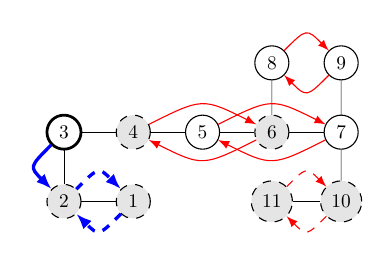
\begin{tikzpicture}[scale=0.22, sibling distance=0em,
  every node/.style = {scale=0.7, shape=circle, draw, align=center},
    outline/.style={draw=#1,thick,fill=#1!100}]
  every draw/.style = {scale=1,thin}
  
  \node[dashed, fill=black!10] (node1) at (4,-4) {1};
  \node[dashed, fill=black!10] (node2) at (0,-4) {2};
  \node[line width=1pt] (node3) at (0,0) {3};
  \node[dashed, fill=black!10] (node4) at (4,0) {4};
  \node[] (node5) at (8,0) {5};
  \node[dashed, fill=black!10] (node6) at (12,0) {6};
  \node[] (node7) at (16,0) {7};
  \node[] (node8) at (12,4) {8};
  \node[] (node9) at (16,4) {9};
  \node[dashed, fill=black!10] (node10) at (16,-4) {10};
  \node[dashed, fill=black!10] (node11) at (12,-4) {11};
  \draw[very thin] (node1)--(node2);
  \draw[very thin] (node2)--(node3);
  \draw[very thin] (node3)--(node4);
  \draw[very thin] (node4)--(node5);
  \draw[very thin] (node5)--(node6);
  \draw[very thin] (node6)--(node7);
  \draw[very thin] (node6)--(node8);
  \draw[very thin] (node7)--(node9);
  \draw[very thin] (node7)--(node10);
  \draw[very thin] (node10)--(node11);
  
%  \draw[-latex,blue,very thick] (node1).. controls(10,-2) ..(node10);
%  \draw[-latex,red] (node2).. controls(3,-3) ..(node4);
  \draw[-{Latex[length=2mm]},blue,very thick] (node3).. controls(-2,-2) ..(node2);
  \draw[-latex,red] (node4).. controls(8,2) ..(node6);
  \draw[-latex,red] (node5).. controls(12,2) ..(node7);
  \draw[-latex,red] (node6).. controls(8,-2) ..(node4);
  \draw[-latex,red] (node7).. controls(12,-2) ..(node5);
  \draw[-latex,red] (node8).. controls(14,6) ..(node9);
  \draw[-latex,red] (node9).. controls(14,2) ..(node8);
%  \draw[-latex,red] (node10).. controls(8,-6) ..(node2);
%  \draw[-latex,blue,very thick] (node11).. controls(6,-6) ..(node2);
  \draw[-{Latex[length=2mm]},blue,very thick,dashed] (node1).. controls(2,-6) ..(node2);
  \draw[-{Latex[length=2mm]},blue,very thick,dashed] (node2).. controls(2,-2) ..(node1);
%  \draw[-latex,red,dashed] (node3).. controls(-1,2) and (1,2) ..(node3);
  \draw[-latex,red,dashed] (node10).. controls(14,-6) ..(node11);
  \draw[-latex,red,dashed] (node11).. controls(14,-2) ..(node10);

\end{tikzpicture}


\end{minipage}
}
\subfigure[]{
\centering
\begin{minipage}[t]{0.3\linewidth}
\centering
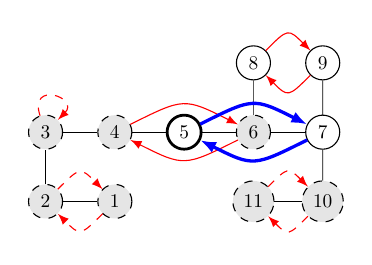
\begin{tikzpicture}[scale=0.22, sibling distance=0em,
  every node/.style = {scale=0.7, shape=circle, draw, align=center},
    outline/.style={draw=#1,thick,fill=#1!100}]
  every draw/.style = {scale=1,thin}
  
  \node[dashed, fill=black!10] (node1) at (4,-4) {1};
  \node[dashed, fill=black!10] (node2) at (0,-4) {2};
  \node[dashed, fill=black!10] (node3) at (0,0) {3};
  \node[dashed, fill=black!10] (node4) at (4,0) {4};
  \node[line width=1pt] (node5) at (8,0) {5};
  \node[dashed, fill=black!10] (node6) at (12,0) {6};
  \node[] (node7) at (16,0) {7};
  \node[] (node8) at (12,4) {8};
  \node[] (node9) at (16,4) {9};
  \node[dashed, fill=black!10] (node10) at (16,-4) {10};
  \node[dashed, fill=black!10] (node11) at (12,-4) {11};
  \draw[very thin] (node1)--(node2);
  \draw[very thin] (node2)--(node3);
  \draw[very thin] (node3)--(node4);
  \draw[very thin] (node4)--(node5);
  \draw[very thin] (node5)--(node6);
  \draw[very thin] (node6)--(node7);
  \draw[very thin] (node6)--(node8);
  \draw[very thin] (node7)--(node9);
  \draw[very thin] (node7)--(node10);
  \draw[very thin] (node10)--(node11);
  
%  \draw[-latex,blue,very thick] (node1).. controls(10,-2) ..(node10);
%  \draw[-latex,red] (node2).. controls(3,-3) ..(node4);
%  \draw[-latex,red] (node3).. controls(-2,-2) ..(node2);
  \draw[-latex,red] (node4).. controls(8,2) ..(node6);
  \draw[-{Latex[length=2mm]},blue,very thick] (node5).. controls(12,2) ..(node7);
  \draw[-latex,red] (node6).. controls(8,-2) ..(node4);
  \draw[-{Latex[length=2mm]},blue,very thick] (node7).. controls(12,-2) ..(node5);
  \draw[-latex,red] (node8).. controls(14,6) ..(node9);
  \draw[-latex,red] (node9).. controls(14,2) ..(node8);
%  \draw[-latex,red] (node10).. controls(8,-6) ..(node2);
%  \draw[-latex,red] (node11).. controls(6,-6) ..(node2);
  \draw[-latex,red,dashed] (node1).. controls(2,-6) ..(node2);
  \draw[-latex,red,dashed] (node2).. controls(2,-2) ..(node1);
  \draw[-latex,red,dashed] (node3).. controls(-1,3) and (2,2) ..(node3);
  \draw[-latex,red,dashed] (node10).. controls(14,-6) ..(node11);
  \draw[-latex,red,dashed] (node11).. controls(14,-2) ..(node10);

\end{tikzpicture}


\end{minipage}
}
\medskip
\subfigure[]{
\centering
\begin{minipage}[t]{0.3\linewidth}
\centering
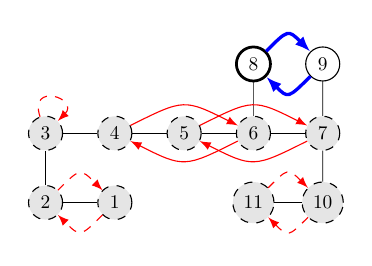
\begin{tikzpicture}[scale=0.22, sibling distance=0em,
  every node/.style = {scale=0.7, shape=circle, draw, align=center},
    outline/.style={draw=#1,thick,fill=#1!100}]
  every draw/.style = {scale=1,thin}
  
  \node[dashed, fill=black!10] (node1) at (4,-4) {1};
  \node[dashed, fill=black!10] (node2) at (0,-4) {2};
  \node[dashed, fill=black!10] (node3) at (0,0) {3};
  \node[dashed, fill=black!10] (node4) at (4,0) {4};
  \node[dashed, fill=black!10] (node5) at (8,0) {5};
  \node[dashed, fill=black!10] (node6) at (12,0) {6};
  \node[dashed, fill=black!10] (node7) at (16,0) {7};
  \node[line width=1pt] (node8) at (12,4) {8};
  \node[] (node9) at (16,4) {9};
  \node[dashed, fill=black!10] (node10) at (16,-4) {10};
  \node[dashed, fill=black!10] (node11) at (12,-4) {11};
  \draw[very thin] (node1)--(node2);
  \draw[very thin] (node2)--(node3);
  \draw[very thin] (node3)--(node4);
  \draw[very thin] (node4)--(node5);
  \draw[very thin] (node5)--(node6);
  \draw[very thin] (node6)--(node7);
  \draw[very thin] (node6)--(node8);
  \draw[very thin] (node7)--(node9);
  \draw[very thin] (node7)--(node10);
  \draw[very thin] (node10)--(node11);
  
%  \draw[-latex,blue,very thick] (node1).. controls(10,-2) ..(node10);
%  \draw[-latex,red] (node2).. controls(3,-3) ..(node4);
%  \draw[-latex,red] (node3).. controls(-2,-2) ..(node2);
  \draw[-latex,red] (node4).. controls(8,2) ..(node6);
  \draw[-latex,red] (node5).. controls(12,2) ..(node7);
  \draw[-latex,red] (node6).. controls(8,-2) ..(node4);
  \draw[-latex,red] (node7).. controls(12,-2) ..(node5);
  \draw[-{Latex[length=2mm]},blue,very thick] (node8).. controls(14,6) ..(node9);
  \draw[-{Latex[length=2mm]},blue,very thick] (node9).. controls(14,2) ..(node8);
%  \draw[-latex,red] (node10).. controls(8,-6) ..(node2);
%  \draw[-latex,red] (node11).. controls(6,-6) ..(node2);
  \draw[-latex,red,dashed] (node1).. controls(2,-6) ..(node2);
  \draw[-latex,red,dashed] (node2).. controls(2,-2) ..(node1);
  \draw[-latex,red,dashed] (node3).. controls(-1,3) and (2,2) ..(node3);
  \draw[-latex,red,dashed] (node10).. controls(14,-6) ..(node11);
  \draw[-latex,red,dashed] (node11).. controls(14,-2) ..(node10);

\end{tikzpicture}


\end{minipage}
}
\subfigure[]{
\centering
\begin{minipage}[t]{0.3\linewidth}
\centering
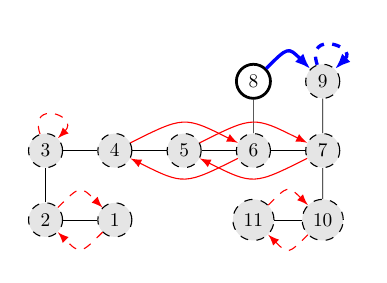
\begin{tikzpicture}[scale=0.22, sibling distance=0em,
  every node/.style = {scale=0.7, shape=circle, draw, align=center},
    outline/.style={draw=#1,thick,fill=#1!100}]
  every draw/.style = {scale=1,thin}
  
  \node[dashed, fill=black!10] (node1) at (4,-4) {1};
  \node[dashed, fill=black!10] (node2) at (0,-4) {2};
  \node[dashed, fill=black!10] (node3) at (0,0) {3};
  \node[dashed, fill=black!10] (node4) at (4,0) {4};
  \node[dashed, fill=black!10] (node5) at (8,0) {5};
  \node[dashed, fill=black!10] (node6) at (12,0) {6};
  \node[dashed, fill=black!10] (node7) at (16,0) {7};
  \node[line width=1pt] (node8) at (12,4) {8};
  \node[dashed, fill=black!10] (node9) at (16,4) {9};
  \node[dashed, fill=black!10] (node10) at (16,-4) {10};
  \node[dashed, fill=black!10] (node11) at (12,-4) {11};
  \draw[very thin] (node1)--(node2);
  \draw[very thin] (node2)--(node3);
  \draw[very thin] (node3)--(node4);
  \draw[very thin] (node4)--(node5);
  \draw[very thin] (node5)--(node6);
  \draw[very thin] (node6)--(node7);
  \draw[very thin] (node6)--(node8);
  \draw[very thin] (node7)--(node9);
  \draw[very thin] (node7)--(node10);
  \draw[very thin] (node10)--(node11);
  
%  \draw[-latex,red] (node1).. controls(10,-2) ..(node10);
%  \draw[-latex,red] (node2).. controls(3,-3) ..(node4);
%  \draw[-latex,red] (node3).. controls(-2,-2) ..(node2);
  \draw[-latex,red] (node4).. controls(8,2) ..(node6);
  \draw[-latex,red] (node5).. controls(12,2) ..(node7);
  \draw[-latex,red] (node6).. controls(8,-2) ..(node4);
  \draw[-latex,red] (node7).. controls(12,-2) ..(node5);
  \draw[-{Latex[length=2mm]},blue,very thick] (node8).. controls(14,6) ..(node9);
%  \draw[-latex,blue,very thick] (node9).. controls(14,2) ..(node8);
%  \draw[-latex,red] (node10).. controls(8,-6) ..(node2);
%  \draw[-latex,red] (node11).. controls(6,-6) ..(node2);
  \draw[-latex,red,dashed] (node1).. controls(2,-6) ..(node2);
  \draw[-latex,red,dashed] (node2).. controls(2,-2) ..(node1);
  \draw[-latex,red,dashed] (node3).. controls(-1,3) and (2,2) ..(node3);
  \draw[-latex,red,dashed] (node10).. controls(14,-6) ..(node11);
  \draw[-latex,red,dashed] (node11).. controls(14,-2) ..(node10);
  \draw[-{Latex[length=2mm]},blue,very thick,dashed] (node9).. controls(15,7) and (18,6) ..(node9);

\end{tikzpicture}


\end{minipage}
}
\subfigure[]{
\centering
\begin{minipage}[t]{0.3\linewidth}
\centering
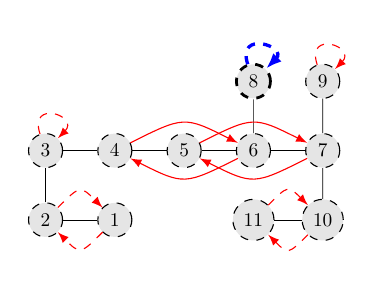
\begin{tikzpicture}[scale=0.22, sibling distance=0em,
  every node/.style = {scale=0.7, shape=circle, draw, align=center},
    outline/.style={draw=#1,thick,fill=#1!100}]
  every draw/.style = {scale=1,thin}
  
  \node[dashed, fill=black!10] (node1) at (4,-4) {1};
  \node[dashed, fill=black!10] (node2) at (0,-4) {2};
  \node[dashed, fill=black!10] (node3) at (0,0) {3};
  \node[dashed, fill=black!10] (node4) at (4,0) {4};
  \node[dashed, fill=black!10] (node5) at (8,0) {5};
  \node[dashed, fill=black!10] (node6) at (12,0) {6};
  \node[dashed, fill=black!10] (node7) at (16,0) {7};
  \node[line width=1pt,dashed, fill=black!10] (node8) at (12,4) {8};
  \node[dashed, fill=black!10] (node9) at (16,4) {9};
  \node[dashed, fill=black!10] (node10) at (16,-4) {10};
  \node[dashed, fill=black!10] (node11) at (12,-4) {11};
  \draw[very thin] (node1)--(node2);
  \draw[very thin] (node2)--(node3);
  \draw[very thin] (node3)--(node4);
  \draw[very thin] (node4)--(node5);
  \draw[very thin] (node5)--(node6);
  \draw[very thin] (node6)--(node7);
  \draw[very thin] (node6)--(node8);
  \draw[very thin] (node7)--(node9);
  \draw[very thin] (node7)--(node10);
  \draw[very thin] (node10)--(node11);
  
%  \draw[-latex,red] (node1).. controls(10,-2) ..(node10);
%  \draw[-latex,red] (node2).. controls(3,-3) ..(node4);
%  \draw[-latex,red] (node3).. controls(-2,-2) ..(node2);
  \draw[-latex,red] (node4).. controls(8,2) ..(node6);
  \draw[-latex,red] (node5).. controls(12,2) ..(node7);
  \draw[-latex,red] (node6).. controls(8,-2) ..(node4);
  \draw[-latex,red] (node7).. controls(12,-2) ..(node5);
%  \draw[-latex,blue,very thick] (node8).. controls(14,6) ..(node9);
%  \draw[-latex,blue,very thick] (node9).. controls(14,2) ..(node8);
%  \draw[-latex,red] (node10).. controls(8,-6) ..(node2);
%  \draw[-latex,red] (node11).. controls(6,-6) ..(node2);
  \draw[-latex,red,dashed] (node1).. controls(2,-6) ..(node2);
  \draw[-latex,red,dashed] (node2).. controls(2,-2) ..(node1);
  \draw[-latex,red,dashed] (node3).. controls(-1,3) and (2,2) ..(node3);
  \draw[-latex,red,dashed] (node10).. controls(14,-6) ..(node11);
  \draw[-latex,red,dashed] (node11).. controls(14,-2) ..(node10);
  \draw[-{Latex[length=2mm]},blue,very thick,dashed] (node8).. controls(11,7) and (14,6) ..(node8);
  \draw[-latex,red,dashed] (node9).. controls(15,7) and (18,6) ..(node9);

\end{tikzpicture}


\end{minipage}
}
\caption{A running example for our mechanism. Though $G(\theta')$ is a directed graph, we omit the double arrows here to make the figure clearer. The single arrows represent the pointing for each agent. The blue lines highlight the pointing of the path under consideration, and the start of the path is marked. The settled agent set is dashed and in grey.}
\label{fig:run_example}
\end{figure*}



\begin{enumerate}
    % \item[(a)] At the beginning, we detect the connected-cycles $C_6=(4,6)$ and $C_7=(5,7)$. Add $C_6$ and $C_7$ to $V$, and connect their neighbors ${3,8,9,10}$ in $G(\theta')$. Since agent 2 is in $N \setminus V$ and agent $4$ is in $V$, change $\langle 2,4\rangle $ to $\langle 2,\succ_2^{next}(F(\theta'))=1\rangle $. 
    
    % Now we detect another connected-cycle $C_9=(8,9)$. Add $C_9$ to $V$ and connect their neighbors ${3,10}$ in $G(\theta')$.
    \item[(a)] At the beginning, agent 1 has 0 in-degree and the minimum order. The path is $P_1=(1,10,2,4,6)$. Since $C_6=(4,6)$ is a dependent connected-cycle, add $C_6$ to $V$. Since agent 2 is in $N \setminus V$ and agent $4$ is in $V$, change $\langle 2,4\rangle $ to $\langle 2,\succ_2^{next}(F(\theta'))=1\rangle $. 
    \item[(b)] Then agent 3 has 0 in-degree and the minimum order, the path is $P_3=(3,2,1,10)$. Since $C_{10}=(2,1,10)$ is an unconnected-cycle and no connected component containing $10$ and $2$ in $G(\theta')$ is a subset of $C_{10}$, change $\langle 10,2\rangle $ to $\langle 10,\succ_{10}^{next}(F(\theta'))=11\rangle $.
    \item[(c)] Agent 3 still has 0 in-degree and the minimum order. The path is $P_3=(3,2,1,10,11)$. Since $C_{11}=(2,1,10,11)$ is an unconnected-cycle and no connected component containing $11$ and $2$ in $G(\theta')$ is a subset of $C_{11}$, change $\langle 11,2\rangle $ to $\langle 11,\succ_{11}^{next}(F(\theta'))=10\rangle $.
    \item[(d)] Agent 3 still has 0 in-degree and the minimum order. The path is $P_3=(3,2,1,10,11)$. Since $C_{11}=(10,11)$ is an independent connected-cycle, add $C_{11}$ to $V$. Since agent 1 is in $N \setminus V$ and agent $10$ is in $V$, change $\langle 1,10\rangle $ to $\langle 1,\succ_{1}^{next}(F(\theta')=2\rangle $
    \item[(e)] Agent 3 still has 0 in-degree and the minimum order. The path is $P_3=(3,2,1)$. Since $C_1=(2,1)$ is an independent connected-cycle, add $C_1$ to $V$. Since agent $3$ is in $N \setminus V$ and agent $2$ is in $V$, change $\langle 3,2\rangle $ to $\langle 3,\succ_{3}^{next}(F(\theta'))=3\rangle $. 
    \item[(f)] No agent in $F(\theta')$ has 0 in-degree. Agent $3$ has the minimum order in $N \setminus V$. The path is $P_3=(3)$. Since $C_3=(3)$ is an independent connected-cycle, add $C_3$ to $V$.
    
    No agent in $F(\theta')$ has 0 in-degree. Agent $5$ has the minimum order in $N \setminus V$. The path is $P_5=(5,7)$. Since $C_7=(5,7)$ is a dependent connected-cycle, add $C_7$ to $V$.
    \item[(g)] No agent in $F(\theta')$ has 0 in-degree. Agent $8$ has the minimum order in $N \setminus V$. The path is $P_8=(8,9)$. Since $C_9=(8,9)$ is an unconnected-cycle and no connected component containing $9$ and $8$ in $G(\theta')$ is a subset of $C_{9}$, change $\langle 9,8\rangle $ to $\langle 9,\succ_9^{next}(F(\theta'))=9\rangle $.
    \item[(h)] Now agent 8 has 0 in-degree and the minimum order. The path is $P_8=(8,9)$. Since $C_9=(9)$ is an independent connected-cycle, add $C_9$ to $V$. Since agent 8 is in $N \setminus V$ and agent 9 is in $V$, change $\langle 8,9\rangle $ to $\langle 8,\succ_8^{next}(F(\theta'))=8\rangle $. 
    \item[(i)] No agent in $F(\theta')$ has 0 in-degree. Agent $8$ has the minimum order in $N \setminus V$. The path is $P_8=(8)$. Since $C_8$ is an independent connected-cycle, add $C_8$ to $V$. 
    
    Now $V = N$, the mechanism ends.
\end{enumerate}



%%%%%%%%%%%%%%%%%%%%%%%%%%%%%%%%%%%%%%%%%%%%%%%%%%%%%%%%%%%%%%%%%%%%%%%%
\section{Properties of CTC}

In this section, we prove that Connected Trading Cycles (CTC) is IR, IC, optimal-c and stable-cc. As shown in Table~\ref{tab:mechanism}, all previous mechanisms fail to satisfy optimal-c, and CTC reaches the theoretical boundaries.
\begin{table}[ht]
\centering
\begin{tabular}{|c|c|c|c|c|}
    \hline
    \multirow{2}{*}{Mechanism} & \multirow{2}{*}{Optimal-c}& \multirow{2}{*}{Stable-cc} & \multicolumn{2}{c|}{IC} \\ \cline{4-5} 
     & & & Trees & All Networks\\ \hline
    TTC~\cite{shapley1974cores} &\ding{53} & \ding{53}& \ding{53} & \ding{53} \\ \hline
    SWN~\cite{Leave_and_Share} & \ding{53} &\ding{51} & \ding{51} & \ding{51} \\ \hline
    SWC~\cite{DBLP:conf/atal/KawasakiWTY21} & \ding{53} &\ding{51}(Trees) & \ding{51} & \ding{53} \\ \hline
    LS~\cite{Leave_and_Share}  & \ding{53} &\ding{51} & \ding{51} & \ding{51} \\ \hline
    \textcolor{red}{CTC}  & \textcolor{red}{\ding{51}} &\textcolor{red}{\ding{51}} & \textcolor{red}{\ding{51}} & \textcolor{red}{\ding{51}} \\ \hline
\end{tabular}
\caption{Comparison on one-sided matching mechanisms over social networks.}
\label{tab:mechanism}
\end{table}

\begin{theorem}
For any order $\mathcal{O}$, CTC is IR.
\end{theorem}
\begin{proof}
In CTC, every agent $i$ can point to her own item $h_i$. When $i$ does so, $i$'s pointing to herself is an independent connected-cycle and our mechanism will assign $h_i$ to $i$. So, CTC is IR. 
\end{proof}

\begin{theorem} 
For any order $\mathcal{O}$, CTC is IC.
\end{theorem}
\begin{proof}
%First of all, we show that the transformation on graph does not violate IC. For those who are matched during the graph transformation procedure, they have been allocated their best allocation, so they have no incentive to misreport. Moreover, since they already get their favorite, they do not care about the rest of the graph, so sharing their neighbors does not affect IC as well. For those who are not matched during the graph transformation procedure, they cannot influence the matched agents, since are connected to each other, regardless of other agents' reported type.

We first consider the truthfulness of agent's report on preference under any given neighbor set report. Suppose $\pi_i(((\succ_i,r_i'),\theta_{-i}'))=h_j$, $\pi_i(((\succ_i',r_i'),\theta_{-i}'))=h_{j'}$, and $h_{j'}\succ_i h_j$. Assume agent $q$ is allocated $h_{j'}$ when agent $i$ truthfully reports preference. Then there exists a connected-cycle $C_1$ involving $\langle q,j'\rangle $. Since $\pi_i(((\succ_i',r_i'),\theta_{-i}'))=h_{j'}$, there exists another connected-cycle $C_2$ involving $\langle i,j'\rangle $. Thus, there must exist an agent $t$ on both $C_1$ and $C_2$ whose pointing is different. Let the two pointing be $\langle t,t_1\rangle , t_1 \in C_1$ and $\langle t,t_2\rangle , t_2 \in C_2$. Given that $q$ is allocated $h_{j'}$ when agent $i$ truthfully reports preference, $C_1$ forms which means $h_{t_1} \succ'_t h_{t_2}$. Similarly, since agent $i$ is allocated $h_{j'}$ when she misreports, $C_2$ forms which means $h_{t_2} \succ'_t h_{t_1}$. This is a contradiction since each agent has a strict preference. Hence, regardless of the report on neighbor set, truthfully reporting preference is a dominant strategy for all agents.

Then we consider the truthfulness of agent's report on neighbor set under any given preference report. Suppose $\pi_i(((\succ'_i,r_i),\theta_{-i}'))=h_j$,  $\pi_i(((\succ'_i,r_i'),\theta_{-i}'))=h_{j'}$, and $h_{j'}\succ'_i h_j$. So, there exists a connected-cycle $C_1$ involving $\langle i,j'\rangle $ when $i$ misreports as $(\succ'_i,r'_i)$. By the definition of connected-cycles, $i$ and $j'$ are involved in a connected component $S$ where no subset of agents in $S$ forms a connected-cycle. Since $h_{j'}\succ'_i h_j$, when truthfully reporting neighbor set, $i$ must have pointed $\langle i,j'\rangle $ before $\langle i,j\rangle $ and is forced to switch to the next on her preference. This indicates that the cycle $C_2$ involving $\langle i,j'\rangle $ when $i$ reports $(\succ'_i,r_i)$ is an unconnected-cycle. Note that the difference in these two cases is caused by $i$ misreporting $r'_i$. If some agents are unqualified because of $i$'s misreporting, it means they can only connect to others by $i$, so their joining in the match cannot change the fact that $\langle i,j'\rangle $ can be involved in a connected-cycle. On the other hand, if no agent becomes unqualified because of $i$'s misreporting, $i$ misreports as $(\succ'_i,r'_i)$ can only decrease her connection to others which is not beneficial. Hence, if $i$ is allocated $h_j'$ when misreporting neighbor set, $i$ can also get $h_j'$ when she truthfully reports which contradicts our assumption. Though misreporting on neighbor set can have impact on the order, with the truthfully reported preferences, whether a cycle can get traded is only determined by the connections as shown above. The changes in the order cannot influence the allocation. Thus, regardless of the preference report, truthfully reporting neighbor set is a dominant strategy for all agents.

% Then we consider the truthfulness of agent's report on neighbor set under truthful preference report. Suppose $\pi_i(((\succ_i,r_i),\theta_{-i}'))=h_j$,  $\pi_i(((\succ_i,r_i'),\theta_{-i}'))=h_{j'}$, and $h_{j'}\succ_i h_j$. So, there exists a connected-cycle $C_1$ involving $\langle i,j'\rangle $ when $i$ misreports as $(\succ_i,r'_i)$. By the definition of connected-cycles, $i$ and $j'$ are involved in a connected component $S$ where no subset of agents in $S$ forms a connected-cycle. Since $h_{j'}\succ_i h_j$, when truthfully reporting neighbor set, $i$ must have pointed $\langle i,j'\rangle $ before $\langle i,j\rangle $ and is forced to switch to the next on her preference. This indicates that the cycle $C_2$ involving $\langle i,j'\rangle $ when $i$ reports $(\succ_i,r_i)$ is an unconnected-cycle. Note that the difference in these two cases is caused by $i$ misreporting $r'_i$. If some agents are unqualified because of $i$'s misreporting, it means they can only connect to others by $i$, so their joining in the match cannot change the fact that $\langle i,j'\rangle $ can be involved in a connected-cycle. On the other hand, if no agent becomes unqualified because of $i$'s misreporting, $i$ misreports as $(\succ_i,r'_i)$ can only decrease her connection to others which is not beneficial. Hence, if $i$ is allocated $h_j'$ when misreporting neighbor set, $i$ can also get $h_j'$ when she truthfully reports which contradicts our assumption. Though misreporting on neighbor set can have impact on the order, with the truthfully reported preferences, whether a cycle can get traded is only determined by the connections as shown above. The changes in the order cannot influence the allocation. Thus, truthfully reporting neighbor set is a dominant strategy for all agents.

Combining them together, CTC is IC.\end{proof}

% \begin{theorem}
% For any order $\mathcal{O}$, CTC is stable-strict-c.
% \end{theorem}
% \begin{proof}
% For any given type profile $\theta$, if CTC violates stable-strict-c, there exists a group of agents $S$ that forms a connect component in $G(\theta)$, they deviate together and swap among themselves can result in a strictly better allocation $\pi'(\theta)$ for all agents in $S$ compared to $\pi(\theta)$ given by CTC. This means, every agent in $S$ is in a trading cycle in $\pi'(\theta)$. Since $S$ is a connected component, there is at least one connected-cycle in $\pi'(\theta)$. Otherwise, $S$ itself is a connected-cycle. In CTC, all connected-cycles are allowed to get traded, which means the strictly better off agents in $\pi'(\theta)$ are involved in unconnected-cycles. This contradicts with our assumption that strictly better off agents form a connected component. Thus, CTC is stable-strict-c.
% \end{proof}

% \begin{corollary}
% For any order $\mathcal{O}$, CTC is optimal-c.
% \end{corollary}
% \begin{proof}
% In Section 4, Theorem 4.4, we prove that if $\pi$ is stable-strict-c, $\pi$ is optimal-c. From Theorem 6.3, we can derive that CTC is also optimal-c.
% \end{proof}



\begin{theorem}
For any order $\mathcal{O}$, CTC is optimal-c. 
\end{theorem}
\begin{proof}
For any given type profile $\theta$, if CTC violates optimal-c, there exists a connected component $T\subseteq N$, with the allocation $\pi(\theta)$ given by CTC, a reallocation $\pi'(\theta)$ among $T$ based on $\pi(\theta)$ makes every agent in $T$ strictly better. We construct a cycle set $\mathbb{C}$ which consists of the cycles given by $\pi$ involving agents in $T$. By the rule of CTC, all the cycles in $\mathbb{C}$ are connected-cycles. We denote the reallocation cycle set given by $\pi'(\theta)$ as $\mathbb{C}^*$. By definition of connected-cycles, since $T$ is a connected component there exists at least one connected-cycle in $\mathbb{C}^*$. Otherwise, $\mathbb{C}^*$ itself is a connected-cycle. For each connected-cycle $C_T$ in $\mathbb{C}^*$, we let each agent $i$ on the cycle switch her pointing to the owner of $\pi'_i(\theta)$. We denote all the cycles changed in $\mathbb{C}$ as $\mathbb{C}_i\subseteq\mathbb{C}$ and they change to $\mathbb{C}_i^*$. Since all cycles in $\mathbb{C}_i$ are changed, every cycle in $\mathbb{C}_i^*$ involves at least one agent in $C_T$. Given that $C_T$ is a connected-cycle and all cycles in $\mathbb{C}_i$ are connected-cycles, all cycles in $\mathbb{C}_i^*$ are connected-cycles. Thus, $\mathbb{C}_i^*\subseteq\mathbb{C}$, which means $\pi=\pi'$ for all agents in $\mathbb{C}_i^*$. By the assumption, the strictly better off group $T$ does not contain these connected-cycles. Hence, all the cycles in $\mathbb{C}^*$ are unconnected-cycles. This means agents in $T$ cannot form a connected component in $G(\theta)$ which contradicts our assumption. Thus, CTC is optimal-c.\end{proof}

\begin{theorem}
For any order $\mathcal{O}$, CTC is stable-cc.
\end{theorem}

\begin{proof}
For any given type profile $\theta$, if CTC violates stable-cc, there exists a group of agents $S$ that forms a complete component in $G(\theta)$, they deviate together and swap among themselves can result in a better allocation $\pi'(\theta)$ compared to $\pi(\theta)$ given by CTC. Since group $S$ is a complete component, all the cycles formed in $\pi'(\theta)$ are independent connected-cycles. In CTC, all these cycles are allowed to get traded. That is to say, CTC will assign them exactly $\pi'$, which contradicts our assumption. Hence, CTC is stable-cc.
\end{proof}

%%%%%%%%%%%%%%%%%%%%%%%%%%%%%%%%%%%%%%%%%%%%%%%%%%%%%%%%%%%%%%%%%%%%%%%
% \section{Discussion}
% Throughout all the IC mechanisms, we observe a pattern commonly shared. We first take a closer look at Connected Trading Cycles. 

% However, TTC fails to 
%If agent $i$ reports $(\succ'_i,r'_i)$ and her allocation is $h_{j'} = \pi_i((\succ'_i,r'_i),\theta'_{-i})$. Let agent $i$ move $h_{j'}$ to a higher rank in $\succ'_i$, we denote the new preference as $\succ''_i$. Since only connected-cycles get traded in CTC, all items $T$ with a higher rank than $h_{j'}$ in $\succ'_i$ are in connected-cycles without agent $i$. By the construction of $\succ''_i$, all items $T'$ with a higher rank than $h_{j'}$ in $\succ''_i$ is a subset of $T$. Thus, $i$ also cannot get items in $T'$, and $h_{j'} = \pi_i((\succ''_i,r'_i),\theta'_{-i})$. In addition, if agent $i$ reports $(\succ'_i,r''_i)$ and her allocation is $h_{q} = \pi_i((\succ'_i,r''_i),\theta'_{-i})$, her allocation is at least $h_{q}$ if she invites more agents ($r''_i\subset r'_i$). 

% \textcolor{red}{Even though a few IC mechanisms have been designed, there is no general explanation why they can satisfy IC property. We are trying to observe the pattern commonly shared by all IC mechanisms, SWN, LS and CTC. According to the definition of incentive compatibility, we can illustrate that the dominant strategy for an agent is truthfully reporting her preference and neighbor set. By the work of~\citeauthor{TAKAMIYA2001201}~\cite{TAKAMIYA2001201}, we find that the monotonicity is relevant to truthfulness over preference. Since neighbor set is the other dimension of agent's type in the network setting other than preference, we conjucture that the preference monotonicity combined with neighbor set monotonicity can be the equvailent form of Incentive Compatibility. Then we try to figure out the monotonicity of each mechanism and give out the definition of monotonicity over two dimensions as well as the proof of equvailence between monotonicity and IC. }
% \begin{theorem}
%     SWN satisfies NS monotonicity.
% \end{theorem}

% \begin{proof}
%     Let's consider $\theta_i'=(\succ_i', r_i')$ and $\theta_i''=(\succ_i', r_i'')$, in which $r_i'' \subseteq r_i'$. We denote the allocated item for $i$ in each type as $\pi_i'$ and $\pi_i''$ respectively.

%     Firstly, $\forall j \in r_i' \setminus r_i''$, there is no edge from $i$ to $j$. As a result, the owner of $\pi_i'$ is in $r_i'$ but may not be in $r_i''$ and the owner of $\pi_i''$ must be in $r_i''$ and $r_i'$. Agent $i$ cannot be allocated $\pi_i'$ by SWN if he reports $\theta_i''$.

%     Secondly, we prove that if 
% \end{proof}
%%%%%%%%%%%%%%%%%%%%%%%%%%%%%%%%%%%%%%%%%%%%%%%%%%%%%%%%%%%%%%%%%%%%%%%%
\section{Incentive Compatible Diffusion One-sided Matching}
%In this section, we present a characterization for incentive compatible diffusion one-sided matching. All existing IC mechanisms fall into our characterization. To begin with, we define the monotonicity of preference, which is first introduced to the housing market by~\citeauthor{TAKAMIYA2001201}~\cite{TAKAMIYA2001201}.

\citeauthor{TAKAMIYA2001201}~\cite{TAKAMIYA2001201} characterizes the strategy-proof housing market mechanisms by preference monotonicity. He shows that with others' preferences fixed, if an agent $i$ gets $h_j$ when reporting $\succ'_i$, she also gets $h_j$ even if $h_j$ is moved to a higher rank in $\succ'_i$.  TTC satisfies this condition since $i$ gets $h_j$ indicating all items better than $h_j$ for agent $i$ are in trading cycles without $i$, and moving $h_j$ to a higher rank will not influence those cycles without $i$. We can easily introduce preference monotonicity into the network setting.

\begin{definition}
    Given agent $i$'s preference profile $\succ_i$ and her allocation $\pi_i$, we denote the set of less preferred items for agent $i$ by $L(\pi_i,\succ_i)=\{k\in H | \pi_i\succ_i k\}$. We say an allocation $\pi$ is \textbf{preference-monotonic} if for any agent $i\in N$, if $L(\pi_i,\succ'_i) \subset L(\pi_i,\succ''_i)$, we have $\pi_i((\succ'_i,r'_i),\theta'_{-i})=\pi_i((\succ''_i,r'_i),\theta'_{-i})$.
\end{definition}

However, preference monotonicity cannot characterize IC in the network setting for it lacks the constraint over the neighbor set report. Let's look back to the house exchange example in the Introduction to get some insights. To incentivize Alice to invite Charlie, we should guarantee that inviting others will not worsen her result. That is, if she can get Bob's house in the Alice-and-Bob market, she can get allocated a house no worse than Bob's when inviting more people. We define this monotonicity of invitation as diffusion monotonicity, which is also studied in the diffusion auction setting~\cite{li2021incentive}.

\begin{definition}
    We say an allocation $\pi$ is \textbf{diffusion-monotonic} if for any agent $i\in N$, if $r''_i \subset r'_i$, we have $\pi_i((\succ'_i,r'_i),\theta'_{-i}) \succeq'_i \pi_i((\succ'_i,r''_i),\theta'_{-i})$.
\end{definition}

Now, we are ready to present the IC characterization for the diffusion one-sided matching.
\begin{theorem}
    A diffusion one-sided matching mechanism is incentive compatible if and only if the allocation $\pi$ is preference-monotonic and diffusion-monotonic.
\end{theorem}
\begin{proof}
Suppose an IC mechanism $\pi$ fails preference-monotonic, then there exists agent $i\in N$ and a preference profile $\succ'_i$ where $L(\pi_i,\succ'_i) \subset L(\pi_i,\succ'_i)$, and we have $h_{j'} = \pi_i((\succ'_i,r'_i)$, $\theta'_{-i})$, $h_j = \pi_i((\succ_i,r'_i),\theta'_{-i})$, $h_j\neq h_{j'}$. Then either $h_{j'}\succ_i h_j$ or $h_j\succ_i h_{j'}$. In the former case, misreporting $\succ'_i$ gives agent $i$ a better allocation and violates IC. In the latter case, $\pi$ fails to be IC when $i$'s true preference is $\succ'_i$. Hence, if a mechanism is IC, it is preference-monotonic.

Similarly, suppose an IC mechanism $\pi$ fails diffusion-monotonic, then there exists agent $i\in N$ and a neighbor set $r'_i$ where $r'_i\subset r_i$, and we have $h_{j'} = \pi_i((\succ'_i,r'_i)$, $\theta'_{-i})$, $h_j = \pi_i((\succ'_i,r_i),\theta'_{-i})$, and $h_{j'}\succ'_i h_j$. In other words, agent $i$ can misreport to make her allocation better, which violates IC. Hence, if a mechanism is IC then it is diffusion-monotonic.

We then prove that if a mechanism is preference-monotonic and diffusion-monotonic, it is IC. That is to say, a mechanism fails IC suggesting that it fails at least one of the monotonicity. If a mechanism $\pi$ is not IC, it means that for at least one agent $i$, she can better her allocation by misreporting her type. If $i$ misreports her neighbor set, the reported $r'_i$ must be a subset of the true neighbor set $r_i$. Thus, $i$ getting a better allocation under $r'_i$ violates diffusion-monotonic. On the other hand, if $i$ misreports her preference profile as $\succ'_i$ to get a better allocation which means $h_{j'} \succ_i h_j$, we will show that this violates preference-monotonic. Let's construct a preference profile $\succ^{*}_i$ for agent $i$, such that the items that ranked first and second in $\succ^{*}_i$ are $h_{j'}$ and $h_j$ respectively. By this construction, we have $L(h_{j'},\succ'_i) \subset L(h_{j'},\succ^{*}_i)$. Since $h_{j'}\succ_i h_j$, we know that $h_{j'} \notin L(h_j,\succ_i)$, so we have $L(h_j,\succ_i) \subset L(h_j,\succ^{*}_i)$. So, if $\pi$ is preference-monotonic, $h_j=h_{j'}$ which contradicts with our assumption.

    To sum up, a diffusion one-sided matching mechanism is IC if and only if it is preference-monotonic and diffusion-monotonic.
\end{proof}


%\textcolor{red}{Next, we provide an example about how to apply our characterization on designing an IC diffusion one-sided matching mechanism. }

Next, we show how to use our characterization to design an IC diffusion one-sided matching mechanism. 

%\textcolor{red}{Should we use a frame for each trivial mechanism? so that this section might seem to be more convincing?}


\begin{figure}[t]
\centering
\subfigure[]{
\centering
\begin{minipage}[t]{0.4\linewidth}
\centering
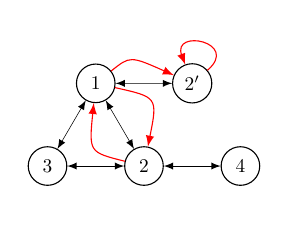
\begin{tikzpicture}[scale=0.35, sibling distance=0em,
  every node/.style = {scale=0.7, shape=circle, draw, align=center,minimum size=0.7cm},
    outline/.style={draw=#1,thick,fill=#1!100}]
  every draw/.style = {scale=1}
  \node (node1) at (1.75,3) {1};
  \node (node2) at (5.25,3) {2$'$};
  \node (node3) at (3.5,0) {2};
  \node[] (node4) at (0,0) {3};
  \node[] (node5) at (7,0) {4};

  
  \draw[latex-latex,very thin] (node1)--(node2);
  \draw[latex-latex,very thin] (node1)--(node3);
  \draw[latex-latex,very thin] (node1)--(node4);
  \draw[latex-latex,very thin] (node3)--(node4);
  \draw[latex-latex,very thin] (node3)--(node5);
  \draw[-latex,red] (node1).. controls(3,4)..(node2);
  \draw[-latex,red] (node1).. controls(4,2.5)..(node3);
  \draw[-latex,white] (node3).. controls(2,-1.5)..(node4);
  \draw[-latex,red] (node3).. controls(1.5,0.5)..(node1);
  \draw[-latex,red] (node2).. controls(7,4.5) and (4.5,5) ..(node2);
\end{tikzpicture}


\end{minipage}
}
\subfigure[]{
\centering
\begin{minipage}[t]{0.4\linewidth}
\centering
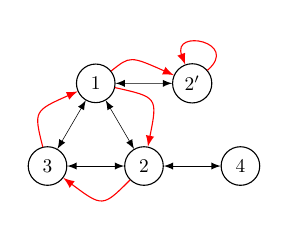
\begin{tikzpicture}[scale=0.35, sibling distance=0em,
  every node/.style = {scale=0.7, shape=circle, draw, align=center,minimum size=0.7cm},
    outline/.style={draw=#1,thick,fill=#1!100}]
  every draw/.style = {scale=2}
  
  %\node[white] (node0) at (-2,0) {};
  \node (node1) at (1.75,3) {1};
  \node (node2) at (5.25,3) {2$'$};
  \node (node3) at (3.5,0) {2};
  \node[] (node4) at (0,0) {3};
  \node[] (node5) at (7,0) {4};

  
  \draw[latex-latex,very thin] (node1)--(node2);
%   \draw[-] (node1)--(node3);
  \draw[latex-latex,very thin] (node1)--(node3);
  \draw[latex-latex,very thin] (node1)--(node4);
  \draw[latex-latex,very thin] (node3)--(node4);
  \draw[latex-latex,very thin] (node3)--(node5);
  \draw[-latex,red] (node1).. controls(3,4)..(node2);
  \draw[-latex,red] (node1).. controls(4,2.5)..(node3);
  \draw[-latex,red] (node3).. controls(2,-1.5)..(node4);
  \draw[-latex,red] (node4).. controls(-0.5,2)..(node1);
  \draw[-latex,red] (node2).. controls(7,4.5) and (4.5,5) ..(node2);

\end{tikzpicture}


\end{minipage}
}

\subfigure[]{
\centering
\begin{minipage}[t]{0.4\linewidth}
\centering
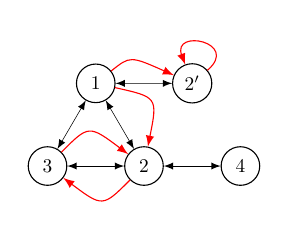
\begin{tikzpicture}[scale=0.35, sibling distance=0em,
  every node/.style = {scale=0.7, shape=circle, draw, align=center,minimum size=0.7cm},
    outline/.style={draw=#1,thick,fill=#1!100}]
  every draw/.style = {scale=2}
  
  %\node[white] (node0) at (-2,0) {};
  \node (node1) at (1.75,3) {1};
  \node (node2) at (5.25,3) {2$'$};
  \node (node3) at (3.5,0) {2};
  \node[] (node4) at (0,0) {3};
  \node[] (node5) at (7,0) {4};

  
  \draw[latex-latex,very thin] (node1)--(node2);
%   \draw[-] (node1)--(node3);
  \draw[latex-latex,very thin] (node1)--(node3);
  \draw[latex-latex,very thin] (node1)--(node4);
  \draw[latex-latex,very thin] (node3)--(node4);
  \draw[latex-latex,very thin] (node3)--(node5);
  \draw[-latex,red] (node1).. controls(3,4)..(node2);
  \draw[-latex,red] (node1).. controls(4,2.5)..(node3);
  \draw[-latex,red] (node3).. controls(2,-1.5)..(node4);
  \draw[-latex,red] (node4).. controls(1.5,1.5)..(node3);
  \draw[-latex,red] (node2).. controls(7,4.5) and (4.5,5) ..(node2);

\end{tikzpicture}


\end{minipage}
}
\subfigure[]{
\centering
\begin{minipage}[t]{0.4\linewidth}
\centering
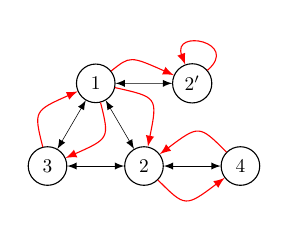
\begin{tikzpicture}[scale=0.35, sibling distance=0em,
  every node/.style = {scale=0.7, shape=circle, draw, align=center,minimum size=0.7cm},
    outline/.style={draw=#1,thick,fill=#1!100}]
  every draw/.style = {scale=1,thin}
  
  %\node[white] (node0) at (-2,0) {};
  \node (node1) at (1.75,3) {1};
  \node (node2) at (5.25,3) {2$'$};
  \node (node3) at (3.5,0) {2};
  \node[] (node4) at (0,0) {3};
  \node[] (node5) at (7,0) {4};

  
  \draw[latex-latex,very thin] (node1)--(node2);
%   \draw[-] (node1)--(node3);
  \draw[latex-latex,very thin] (node1)--(node3);
  \draw[latex-latex,very thin] (node1)--(node4);
  \draw[latex-latex,very thin] (node3)--(node4);
  \draw[latex-latex,very thin] (node3)--(node5);
  \draw[-latex,red] (node1).. controls(3,4)..(node2);
  \draw[-latex,red] (node1).. controls(4,2.5)..(node3);
  \draw[-latex,red] (node3).. controls(5,-1.5)..(node5);
  \draw[-latex,red] (node5).. controls(5.5,1.5)..(node3);
  \draw[-latex,red] (node1).. controls(2.25,1)..(node4);
  \draw[-latex,red] (node4).. controls(-0.5,2)..(node1);
  \draw[-latex,red] (node2).. controls(7,4.5) and (4.5,5) ..(node2);

\end{tikzpicture}


\end{minipage}
}
\caption{Examples for the IC mechanisms designed by monotonicity conditions. Sub-figure (a) depicts the pair-wise mechanism. The other three sub-figures are the extended versions, (d) illustrates SWN.}
\label{fig:characterization}
\end{figure}

Based on the two monotonicity conditions, we construct a simple pair-wise rule. Following a pre-defined order, we let agent 1 with the smallest order choose her favorite neighbor agent 2. If agent 2 finds $h_1$ acceptable, agents 1 and 2 form a trading cycle and get traded. Otherwise, agent 2 leaves with her own item, and agent 1 chooses her next favorite neighbor (as shown in Figure~\ref{fig:characterization} (a)). This trivial mechanism satisfies preference monotonicity since agents always trade with their favorite neighbors that find them acceptable. For diffusion monotonicity, since agents can only choose from their neighbors and the chosen neighbor either accepts the trade or leaves alone, inviting more neighbors guarantees the same, if not better, result.

We can take one step further and extend it to a three-agent version without violating the monotonicity conditions. Whenever an agent chooses her favorite neighbor agent 2, 2 can also choose one from the common neighbors of agents 1 and 2, say agent 3. Now, agent 3 can either choose agent 1 or stay with her own good (as shown in Figure~\ref{fig:characterization} (b)). Notice that, it is also natural to allow agent 3 to choose agent 2, and they can get traded. This is because the neighbor relationship between agents 2 and 3 is irrelevant to others' actions (as shown in Figure~\ref{fig:characterization} (c)). We can further expand this to any size. All agents can choose their favorite among their neighbors (as shown in Figure~\ref{fig:characterization} (d)). By doing so, we no longer need the pre-defined order to determine which agent should leave or trade, since there always exists at least one trading cycle and each agent's allocation is only determined by whether the agent is in a trading cycle or not. Therefore, we can ignore the pre-defined order and then the mechanism is equivalent to SWN.

As shown above, we can first construct a trivial solution that satisfies the monotonicity conditions, and gradually refine it to meet other properties.
%Without the limits on the cycle size, we can ignore the pre-defined order because there will also be a trading cycle when everyone points to her favorite item.
%%%%%%%%%%%%%%%%%%%%%%%%%%%%%%%%%%%%%%%%%%%%%%%%%%%%%%%%%%%%%%%%%%%%%%%%
\section{Conclusion}
This work promotes the theoretical boundary regarding optimality and stability for one-sided matching with initial endowments over social networks. We design the Connected Trading Cycles that satisfies IC, IR, stable-cc, and optimal-c. 
%We prove that stable-strict-c and optimal-c reaches the theoretical boundary in a special graph family, and any given graph can be transformed to such special graph with a transformation procedure (which does not affect the property of the mechanism). 
Furthermore, we propose the first IC characterization in the network setting to complete the theoretical framework. There are still open questions worth investigating in this field. One possible future work is to design diffusion mechanisms for the variants of one-sided matching problems. In addition, the optimal-c solution for diffusion one-sided matching is not unique. How to determine the superiority among different optimal-c allocations and their relationships to one another would be an intriguing research topic. 
%Furthermore, it is also worthwhile to examine how the existing diffusion one-sided matching mechanisms work on real-world data and apply them to solve matching problems in reality.

%%%%%%%%%%%%%%%%%%%%%%%%%%%%%%%%%%%%%%%%%%%%%%%%%%%%%%%%%%%%%%%%%%%%%%%%


% Bibliography
\bibliographystyle{ACM-Reference-Format}
\bibliography{sample-bibliography}

% Appendix
% \appendix
\end{document}

% \section{Comparison and Analysis}
% To the best of our knowledge, we are the first work that focuses on the achievable optimality in the diffusion one-sided matching. Also, the Connected Trading Cycles (CTC) is the only solution that satisfies both stability and optimality boundaries. We wonder how CTC performs in comparison to other mechanisms in simulations. 

% \noindent\textbf{Basic Set-ups}

% There are several criteria used to evaluate different aspects of the mechanisms. In general, we focus on how each criterion evolves along with different connectivity of a social network. We adopt Erdős–Rényi method to generate social networks. Let $n$ represent the node number of a social network. Let $p$ indicate the probability of an edge's existence in the network and a larger $p$ corresponds to a denser network. In particular, when $p=1$ the network is a complete graph. We fix $n=50$ and compare all the diffusion one-sided matching mechanisms in general social networks.

% To begin with, we carry out experiments similar to the ones in~\cite{Leave_and_Share} based on the average ascension for all agents. 

% \noindent\textbf{Criterion 1: Average Ascension}

% We define the ascension for each agent $i$ as follows. Suppose for agent i, the initial endowment $h_i$ is the $j^{th}$ favorite item on her preference and the allocation $\pi_i(\theta)$ given by mechanism $\pi$ is her $k^{th}$ favorite item, then $d_i=j-k$ is $i$'s degree of satisfaction upon $\pi$. We use the average ascension $D = \frac{\sum_{i\in N}d_i}{n}$ to indicate the overall degree of satisfaction regarding a given mechanism. 

% To witness the change of $D$ with different connectivity of the social network, we generate networks with 50 different connectivity $p$ ranging from 0.02 to 1. For each $p$, we compute $D$ upon a random but fixed preference profile in 500 random networks. 


% The result is shown in Figure~\ref{fig:D1}. We adopt the allocation given by TTC as the benchmark of $D$. Note that in the complete graph, all mechanisms provide the same allocation. With the increase of $p$, CTC's allocation converges to the complete graph allocation faster than SWN. Although CTC satisfies optimal-c, its average ascension is worse than LS's when the network is sparse. LS outperforms due to the sharing process among the remaining neighbors after a cycle leaves. In LS, some non-neighbor agents become new neighbors and swap with each other, which is not allowed in CTC. This leads to another observation. When applying LS, agents who have to leave earlier have severely limited selection scope. It seems a bit unfair to them. So we define a more personal criterion called popularity. 

% \begin{figure}[h]
%     \centering
%     \includegraphics[scale=0.2]{50agents_500graphs_D_p_1027.png}
%     \caption{$n$ = 50, 500 networks, 50 different $p$ from 0.02 to 1, to see the change in $D$ of each mechanism.}
%     \label{fig:D1}
% \end{figure}


% \noindent\textbf{Criterion 2: Popularity}

% For the allocation given by different mechanisms, we let each agent vote on her favorite one/ones. We consider the percentage of agents voted for each mechanism as its popularity.

% For 50 different $p$ from 0.02 to 1, we generate 500 random networks and random preference profiles. As show in Figure~\ref{fig:pop500}, CTC is the most popular mechanism for most of the connectivity $p$. All diffusion one-sided matching mechanisms are close to 1 when $p$ is close to 0 because the allocations given by CTC, SWN, or LS are nearly identical in extremely sparse social networks. As the increase of $p$, the popularity of all three mechanisms decreases at first and then increases. Intuitively, low connectivity causes most of the preferred trading cycles to be unconnected, which is not allowed to exist by CTC. However, for LS, the sharing process can add connections between agents, which improves its performance in low connectivity. With the increase of connectivity, all mechanisms converge to the allocation in a complete graph, so agents vote for them equally.
% % Some agents prefer the allocation given by CTC and some agents do not.
% %CTC outperforms the other two and converges to TTC faster.

% %Another intriguing phenomenon is that the popularity of the 

% %cannot be compatible with IC, a major set of agents cannot be allocated their preferred items in diffusion mechanisms when the connectivity is low. However, some others might be able to match with preferred items, even better than TTC. 

% % (same as the allocation given by TTC)
% %So, they vote for the diffusion mechanisms over TTC. 


% Next, we use rank maximality, a practical optimality criterion for matching to evaluate the performances of the mechanisms.
% %An alternative practical optimality criterion for matching is rank maximality.

% \begin{figure}[t]
%     \centering
%     \includegraphics[scale=0.2]{popularity_500graphs_withoutTTC.png}
%     \caption{$n$ = 50, 500 networks, 50 different $p$ from 0.02 to 1, to see the popularity of each mechanism.}
%     \label{fig:pop500}
% \end{figure}
% \begin{figure}[t]
%     \centering
%     \includegraphics[scale=0.2]{50agents_500graphs_RankMaximal_p_1027_0.02.png}
%     \caption{$n$ = 50, 2000 networks, 50 different $p$ from 0.02 to 1, to see the rank maximality times of each mechanism.}
%     \label{fig:rank2000}
% \end{figure}

% \noindent\textbf{Criterion 3: Rank Maximality}

% Rank maximality regards a mechanism as a better one if more agents are matched with their top choice. We count the number of agents regarding the preference rank of one’s allocation under different mechanisms. In the simulation, we generate 2000 random networks with different connectivity $p$. For each network, the preference profiles are also randomly generated. For each $p$ from 0.02 to 1, we compute the rank maximality times for each mechanism.  
% %Here, we opt out TTC because when the connectivity is low, TTC will always be the rank maximal mechanism leaving us no chance to investigate which diffusion mechanism performs better.

% The result depicted in Figure~\ref{fig:rank2000} shows LS performs well in extremely sparse graphs and CTC guarantees its superiority in most of the graphs. The possible reason is that CTC maintains more `favorite trading cycles' since agents' selection scope is not limited.

% Based on the above simulations, Connected Trading Cycles performs better in most connectivity in all three dimensions, i.e., average ascension, popularity and rank maximality. This observation indicates that optimal-c not only is a theoretical optimality notion, but also guarantees a good overall cardinal performance. For Leave and Share, it works well in extremely sparse graphs due to its sharing process. In summary, we should apply LS in extremely sparse networks and CTC in the others to reach a better outcome regarding all the three criteria presented. 


% As shown by \citeauthor{kumar2022integration}~\cite{kumar2022integration}, more than half of the participants tend to form a smaller market under TTC. In the traditional setting, mechanism designers do not need to take this into consideration, since the market size is irrelevant to participants' actions. Unfortunately, in the network setting, participants can decide the size of the market through strategic invitations, which causes the incompatibility between IC, stability, and optimality. Hence, we should investigate new theoretical boundaries and design a mechanism to reach them.

%%%%%%%%%%%%%%%%%%%%%%%%%%%%%%%%%%%%%%%%%%%%%%%%%%%%%%%%%%%%%%%%%%%%%%%%
